\documentclass[../main.tex]{subfiles}
\renewcommand{\lop}{PRE}
\graphicspath{{Hinh_PRE1_Tuan14/}{Data_PhieuBaiTap_HK0/Hinh_PRE1_Tuan14/}}
\begin{document}

% Hình dùng chung thư mục của PBT (Data_PhieuBaiTap_HK0/Hinh_PRE1_Tuan14), tên hình có tiền tố p14_
\graphicspath{{Hinh_PRE1_Tuan14/}{Data_PhieuBaiTap_HK0/Hinh_PRE1_Tuan14/}{Data_GiaoAn_HK0/Hinh_PRE1_Tuan14/}{../Data_PhieuBaiTap_HK0/Hinh_PRE1_Tuan14/}}
\raggedbottom % không kéo giãn khoảng trống trên trang khi hình lớn bị đẩy sang trang sau
%=========================================================

%---------- Lệnh dùng riêng cho giáo án ----------
% Nội dung bổ sung / chỉnh sửa (in màu đen như phần còn lại)
\providecommand{\GAbs}{}\renewcommand{\GAbs}[1]{#1}
\definecolor{GAbosung}{HTML}{1F4E79}
% Tiêu đề mục nhỏ trong một hoạt động
\providecommand{\GAmucnho}{}\renewcommand{\GAmucnho}[1]{\par\addvspace{4pt}\noindent{\color{mauchinh}\bfseries #1}\par\nopagebreak\addvspace{2pt}}
% Lời GV / HS nói (in nghiêng, có dấu ngoặc kép)
\providecommand{\GAloi}{}\renewcommand{\GAloi}[1]{\textit{“#1”}}
% Bắt đầu hình ngay dưới đoạn phía trên (không tách trang)
\providecommand{\GAbatdauhinh}{}\renewcommand{\GAbatdauhinh}{\par\nopagebreak\vspace{4pt}\nopagebreak}
% Danh sách gọn (đặt ngay sau \begin{itemize}): giảm khoảng cách giữa các dòng
\providecommand{\GAgon}{}\renewcommand{\GAgon}{\setlength{\itemsep}{4pt}\setlength{\parsep}{0pt}\setlength{\parskip}{0pt}}
% Chèn hình: tranh nào đã vẽ bằng TikZ (danh sách \GAdangky bên dưới) thì vẽ luôn, KHÔNG cần file ảnh;
% tranh khác mới tìm file ảnh, thiếu thì hiện khung "Thiếu hình" (không làm lỗi biên dịch)
%   \GAhinh[tuỳ chọn]{tên đầy đủ}        ví dụ \GAhinh[height=2cm]{p14_de.png}
%   \GAhinhx[tuỳ chọn]{tên không tiền tố} tìm p14_tên rồi ga14_tên, ví dụ \GAhinhx[height=2cm]{ba.png}
\makeatletter
\def\GA@thu#1#2{\ifx\GA@duong\@empty\IfFileExists{#1#2}{\def\GA@duong{#1#2}}{}\fi}
\def\GA@tim#1{%
  \GA@thu{}{#1}\GA@thu{Hinh_PRE1_Tuan14/}{#1}\GA@thu{Data_PhieuBaiTap_HK0/Hinh_PRE1_Tuan14/}{#1}%
  \GA@thu{Data_GiaoAn_HK0/Hinh_PRE1_Tuan14/}{#1}\GA@thu{Hinh_GiaoAn_PRE1_Tuan14/}{#1}%
  \GA@thu{Data_GiaoAn_HK0/Hinh_GiaoAn_PRE1_Tuan14/}{#1}\GA@thu{../Data_PhieuBaiTap_HK0/Hinh_PRE1_Tuan14/}{#1}%
  \GA@thu{Data_GiaoAn_HK0/}{#1}%
  \GA@thu{Data_PhieuBaiTap_HK0/Hinh_PRE1_Tuan14 2/}{#1}\GA@thu{Data_PhieuBaiTap_HK0/Hinh_PRE1_Tuan14 3/}{#1}%
  \GA@thu{Data_PhieuBaiTap_HK0/Hinh_PRE1_Tuan14 4/}{#1}\GA@thu{Data_PhieuBaiTap_HK0/Hinh_PRE1_Tuan14 5/}{#1}}
\def\GA@chen#1#2{\includegraphics[#2]{#1}}
\def\GA@ketqua#1#2{%
  \ifx\GA@duong\@empty
    \edef\GA@ten{#2}\fbox{\parbox{2.2cm}{\centering\scriptsize\color{red}Thiếu hình\\\detokenize\expandafter{\GA@ten}}}%
  \else\expandafter\GA@chen\expandafter{\GA@duong}{#1}\fi}
\providecommand{\GAhinh}{}\renewcommand{\GAhinh}[2][]{%
  \ifcsname GAve@#2\endcsname\GA@vetranh{#1}{#2}\else\def\GA@duong{}\GA@tim{#2}\GA@ketqua{#1}{#2}\fi}
\providecommand{\GAhinhx}{}\renewcommand{\GAhinhx}[2][]{%
  \ifcsname GAve@p14_#2\endcsname\GA@vetranh{#1}{p14_#2}\else\def\GA@duong{}\GA@tim{p14_#2}\GA@tim{ga14_#2}\GA@ketqua{#1}{p14_#2}\fi}
% Đánh lại số bài từ 1 (cho Bài 1, Bài 2 lấy từ PBT)
\providecommand{\GAdatlaibai}{}\renewcommand{\GAdatlaibai}{\@ifundefined{c@bt}{}{\setcounter{bt}{0}}}
\makeatother
% Các lệnh giống PBT PRE1 Tuần 14 (dùng được cả khi không có file PBT trong main)
\providecommand{\TThinh}{}\renewcommand{\TThinh}[2][8cm]{\par\nopagebreak\vspace{2pt}\nopagebreak{\centering\GAhinh[height=#1,width=\linewidth,keepaspectratio]{#2}\par}\vspace{2pt}}
\providecommand{\TTbatdauhinh}{}\renewcommand{\TTbatdauhinh}{\par\nopagebreak\vspace{4pt}\nopagebreak}

%---------- Màu dùng cho hình vẽ (giống PBT PRE1 Tuần 14) ----------
\definecolor{PKdo}{RGB}{230,60,60}\definecolor{PKxanhla}{RGB}{90,180,80}
\definecolor{PKxanhdam}{RGB}{20,90,190}\definecolor{PKvang}{RGB}{255,205,60}
\definecolor{PKvangnhat}{RGB}{255,243,190}\definecolor{PKcam}{RGB}{255,150,60}
\definecolor{PKhong}{RGB}{255,140,180}\definecolor{PKnau}{RGB}{140,85,45}
\definecolor{PKxanhnuoc}{RGB}{90,170,235}
\definecolor{GAkem}{RGB}{255,248,225}\definecolor{GAoli}{RGB}{70,150,220}
\definecolor{GAsau}{RGB}{165,208,100}
\definecolor{GAdochu}{RGB}{238,28,36}\definecolor{GAsoke}{RGB}{25,35,140}

% ===================== TRANH VẼ BẰNG TIKZ (thay cho ảnh) =====================
% Mỗi tranh vẽ quanh gốc toạ độ, khung khoảng [-1.2;1.2] x [-1;1.2]
\tikzset{GAvien/.style={draw=black!60,line width=0.5pt,line join=round,line cap=round}}
% bóng đổ dưới chân: \GAbongdo{x}{y}{rx}
\providecommand{\GAbongdo}{}\renewcommand{\GAbongdo}[3]{\fill[black,opacity=0.13] (#1,#2) ellipse (#3 and #3*0.14);}
% khối tròn có sáng tối (ánh sáng từ trên trái): \GAkhoi{x}{y}{r}{màu}
\providecommand{\GAkhoi}{}\renewcommand{\GAkhoi}[4]{%
  \begin{scope}\clip (#1,#2) circle (#3);
  \shade[inner color=#4!55!white,outer color=#4!75!black] ({#1-0.35*#3},{#2+0.35*#3}) circle ({1.5*#3});\end{scope}
  \draw[#4!45!black,line width=0.45pt] (#1,#2) circle (#3);}
\definecolor{GAda}{RGB}{255,214,180}\definecolor{GAdam}{RGB}{226,160,120}
\definecolor{GAtoc}{RGB}{60,40,30}\definecolor{GAtrau}{RGB}{78,84,96}
\definecolor{GAnaudo}{RGB}{150,85,40}\definecolor{GAxanhla2}{RGB}{70,150,60}
% ---------- con dê ----------
\providecommand{\GAveDe}{}\renewcommand{\GAveDe}{%
  \begin{scope}[GAvien]
  \GAbongdo{0.15}{-0.97}{0.95}
  \foreach \gx in {-0.9,0.2,0.85}{\fill[green!55!black] (\gx-0.15,-0.98) -- (\gx-0.08,-0.75) -- (\gx-0.02,-0.95) -- (\gx+0.04,-0.72) -- (\gx+0.1,-0.95) -- (\gx+0.17,-0.8) -- (\gx+0.2,-0.98) -- cycle;}
  \foreach \gx in {0.78,-0.22}{\filldraw[fill=gray!30] (\gx-0.07,-0.1) rectangle (\gx+0.07,-0.85); \filldraw[fill=black!70] (\gx-0.08,-0.85) rectangle (\gx+0.08,-0.97);}
  \begin{scope}\clip (0.2,0.05) ellipse (0.78 and 0.4); \fill[white] (0.2,0.05) ellipse (0.78 and 0.4);
    \shade[top color=white,bottom color=gray!40] (-0.7,-0.4) rectangle (1.1,0.5);
    \foreach \gx in {-0.4,-0.2,...,0.8}{\draw[gray!45,line width=0.4pt] (\gx,0.15) .. controls (\gx+0.05,0.0) .. (\gx,-0.2);}\end{scope}
  \draw (0.2,0.05) ellipse (0.78 and 0.4);
  \foreach \gx in {0.55,-0.42}{\filldraw[fill=gray!10] (\gx-0.07,-0.15) rectangle (\gx+0.07,-0.88); \filldraw[fill=black!70] (\gx-0.08,-0.88) rectangle (\gx+0.08,-0.99);}
  \filldraw[fill=white] (0.95,0.3) .. controls (1.15,0.45) and (1.15,0.25) .. (1.0,0.15) -- cycle;
  \filldraw[fill=PKhong!60] (0.45,-0.33) ellipse (0.12 and 0.07);
  \filldraw[fill=white] (-0.6,0.25) -- (-0.82,0.62) -- (-0.45,0.72) -- (-0.3,0.3) -- cycle;
  \shade[left color=yellow!55!brown,right color=brown!70!black,draw=brown!50!black,line width=0.4pt] (-0.66,0.84) .. controls (-0.55,1.12) and (-0.25,1.12) .. (-0.16,0.9) .. controls (-0.3,1.0) and (-0.5,0.98) .. (-0.56,0.82) -- cycle;
  \shade[left color=yellow!65!brown,right color=brown!60!black,draw=brown!50!black,line width=0.4pt] (-0.8,0.86) .. controls (-0.72,1.16) and (-0.42,1.2) .. (-0.3,0.98) .. controls (-0.45,1.06) and (-0.62,1.04) .. (-0.7,0.84) -- cycle;
  \shade[inner color=white,outer color=gray!30,rotate around={-30:(-0.78,0.68)}] (-0.78,0.68) ellipse (0.34 and 0.22);
  \draw[rotate around={-30:(-0.78,0.68)}] (-0.78,0.68) ellipse (0.34 and 0.22);
  \filldraw[fill=white,rotate around={25:(-0.48,0.78)}] (-0.42,0.78) ellipse (0.16 and 0.06);
  \fill[PKhong!70,rotate around={25:(-0.48,0.78)}] (-0.42,0.78) ellipse (0.1 and 0.03);
  \filldraw[fill=PKhong!45] (-1.02,0.5) ellipse (0.13 and 0.1);
  \fill[black] (-1.06,0.52) circle (0.018) (-0.98,0.53) circle (0.018);
  \filldraw[fill=white] (-0.95,0.4) -- (-0.85,0.42) -- (-0.92,0.18) -- cycle;
  \fill[black] (-0.8,0.74) circle (0.055); \fill[white] (-0.79,0.76) circle (0.018);
  \draw (-0.98,0.42) .. controls (-0.94,0.38) .. (-0.88,0.42);
  \end{scope}}
% ---------- con cò ----------
\providecommand{\GAveCo}{}\renewcommand{\GAveCo}{%
  \begin{scope}[GAvien]
  \draw[red!75!black,line width=1.6pt] (0.05,-0.2) -- (0.0,-0.55) -- (0.05,-0.97) (0.25,-0.2) -- (0.3,-0.55) -- (0.25,-0.97);
  \draw[red!75!black,line width=1.2pt] (-0.1,-0.97) -- (0.15,-0.97) (0.12,-0.97) -- (0.4,-0.97);
  \filldraw[fill=black!85] (0.45,-0.05) -- (0.95,-0.45) -- (0.62,-0.12) -- (0.9,-0.3) -- (0.55,0.05) -- cycle;
  \GAbongdo{0.15}{-0.98}{0.45}
  \shade[top color=white,bottom color=gray!30,rotate around={-20:(0.2,0.05)}] (0.2,0.05) ellipse (0.48 and 0.27);
  \draw[rotate around={-20:(0.2,0.05)}] (0.2,0.05) ellipse (0.48 and 0.27);
  \filldraw[fill=black!85] (0.25,0.08) .. controls (0.5,0.15) and (0.7,0.0) .. (0.78,-0.25) .. controls (0.55,-0.15) and (0.4,-0.12) .. (0.25,0.08);
  \draw[gray!60] (0.0,0.05) .. controls (0.2,-0.05) .. (0.45,-0.05) (0.05,-0.05) .. controls (0.25,-0.12) .. (0.5,-0.12);
  \draw[gray!80,thin] (0.45,0.0) -- (0.62,-0.18) (0.52,0.05) -- (0.7,-0.12);
  \draw[black!75,line width=7.5pt] (-0.12,0.22) .. controls (-0.3,0.45) and (0.0,0.6) .. (-0.18,0.85);
  \draw[white,line width=6pt] (-0.12,0.22) .. controls (-0.3,0.45) and (0.0,0.6) .. (-0.18,0.85);
  \filldraw[fill=white] (-0.18,0.87) circle (0.13);
  \filldraw[fill=orange!85!red] (-0.27,0.9) -- (-0.85,0.66) -- (-0.26,0.8) -- cycle;
  \fill[black] (-0.2,0.9) circle (0.03);
  \end{scope}}
% ---------- hòn đá ----------
\providecommand{\GAveDa}{}\renewcommand{\GAveDa}{%
  \begin{scope}[GAvien]
  \fill[black!10] (0,-0.62) ellipse (1.2 and 0.12);
  \filldraw[top color=gray!40!brown!25!white,bottom color=gray!75!brown] (-0.75,-0.6) -- (-0.85,-0.2) -- (-0.45,0.15) -- (-0.05,0.05) -- (0.05,-0.6) -- cycle;
  \filldraw[top color=gray!30!white,bottom color=gray!70!black] (-0.2,-0.6) -- (-0.25,0.05) -- (0.2,0.45) -- (0.65,0.25) -- (0.75,-0.6) -- cycle;
  \fill[gray!20] (-0.25,0.05) -- (0.2,0.45) -- (0.3,0.1) -- cycle;
  \filldraw[top color=gray!50!brown!40!white,bottom color=gray!85!black] (0.45,-0.6) -- (0.55,-0.15) -- (0.95,0.0) -- (1.15,-0.6) -- cycle;
  \foreach \gx/\gy/\gr in {-1.05/-0.55/0.12,-0.6/-0.72/0.09,0.3/-0.75/0.1,0.95/-0.72/0.08,-0.15/-0.78/0.07}{\filldraw[fill=gray!55] (\gx,\gy) ellipse (\gr*1.4 and \gr);}
  \draw[gray!75!black,line width=0.4pt] (-0.6,-0.1) -- (-0.45,-0.2) -- (-0.35,-0.35) (0.25,0.2) -- (0.35,0.0) -- (0.45,-0.15) (0.75,-0.2) -- (0.85,-0.4);
  \fill[white,opacity=0.35] (-0.7,-0.15) -- (-0.45,0.1) -- (-0.4,0.0) -- cycle (0.62,-0.12) -- (0.92,-0.02) -- (0.85,-0.1) -- cycle;
  \end{scope}}
% ---------- bé và bể cá ----------
\providecommand{\GAveBeCa}{}\renewcommand{\GAveBeCa}{%
  \begin{scope}[GAvien]
  % bàn và bể cá
  \draw[GAnaudo,line width=2pt] (0.2,-0.25) -- (0.75,-0.98) (0.75,-0.25) -- (0.2,-0.98) (0.47,-0.25) -- (0.47,-0.98);
  \GAbongdo{0.0}{-0.98}{0.95}
  \filldraw[top color=yellow!50!brown!60,bottom color=brown!70!black] (0.47,-0.22) ellipse (0.5 and 0.1);
  \draw[brown!50!black,thin] (0.1,-0.22) .. controls (0.4,-0.18) .. (0.8,-0.23);
  \filldraw[fill=PKxanhnuoc!20,fill opacity=0.9] (0.47,0.15) circle (0.36);
  \begin{scope}\clip (0.47,0.15) circle (0.36); \fill[PKxanhnuoc!55] (0,-0.3) rectangle (1,0.22);
    \fill[yellow!50!brown] (0,-0.3) rectangle (1,-0.12);
    \draw[green!50!black,line width=1.4pt] (0.3,-0.15) .. controls (0.25,0.0) .. (0.32,0.12) (0.65,-0.15) .. controls (0.7,0.0) .. (0.63,0.08);\end{scope}
  \draw (0.47,0.15) circle (0.36);
  \filldraw[fill=PKxanhnuoc!35] (0.47,0.48) ellipse (0.24 and 0.05);
  \filldraw[fill=orange!90] (0.4,0.06) ellipse (0.12 and 0.07); \filldraw[fill=orange!90] (0.52,0.06) -- (0.62,0.12) -- (0.62,0.0) -- cycle;
  \fill[white,opacity=0.6] (0.25,0.3) ellipse (0.05 and 0.1);
  % bé trai
  \filldraw[fill=orange!90] (-0.78,-0.98) rectangle (-0.6,-0.9) (-0.48,-0.98) rectangle (-0.3,-0.9);
  \filldraw[fill=GAda] (-0.72,-0.9) rectangle (-0.62,-0.6) (-0.46,-0.9) rectangle (-0.36,-0.6);
  \filldraw[fill=GAnaudo!80!black] (-0.78,-0.62) -- (-0.8,-0.25) -- (-0.28,-0.25) -- (-0.3,-0.62) -- (-0.5,-0.62) -- (-0.54,-0.45) -- (-0.58,-0.62) -- cycle;
  \filldraw[top color=green!35!white,bottom color=green!55!black!70,rounded corners=4pt] (-0.85,-0.28) -- (-0.88,0.22) -- (-0.22,0.22) -- (-0.25,-0.28) -- cycle;
  \filldraw[fill=green!45!white] (-0.28,0.18) -- (-0.05,0.12) -- (-0.05,0.0) -- (-0.28,0.02) -- cycle;
  \filldraw[fill=GAda] (-0.05,0.1) -- (0.08,0.1) .. controls (0.12,0.2) .. (0.05,0.28) -- (0.02,0.12) -- (-0.05,0.02) -- cycle;
  \filldraw[fill=green!45!white] (-0.85,0.15) -- (-1.0,-0.15) -- (-0.88,-0.2) -- (-0.8,-0.02) -- cycle;
  \filldraw[fill=GAda] (-0.98,-0.17) circle (0.07);
  \begin{scope}\clip (-0.55,0.55) circle (0.32);\fill[white] (-0.55,0.55) circle (0.32);\shade[inner color=GAda!60!white,outer color=GAdam] (-0.65,0.65) circle (0.45);\end{scope}
  \draw (-0.55,0.55) circle (0.32);
  \filldraw[fill=GAtoc] (-0.88,0.62) .. controls (-0.9,0.95) and (-0.3,1.05) .. (-0.22,0.7) .. controls (-0.35,0.78) and (-0.5,0.72) .. (-0.55,0.8) .. controls (-0.62,0.7) and (-0.8,0.72) .. (-0.88,0.62);
  \fill[black] (-0.66,0.56) circle (0.04) (-0.44,0.56) circle (0.04);
  \fill[PKhong!80] (-0.74,0.44) circle (0.05) (-0.36,0.44) circle (0.05);
  \filldraw[fill=red!70!black] (-0.65,0.4) .. controls (-0.6,0.28) and (-0.5,0.28) .. (-0.45,0.4) -- cycle;
  \end{scope}}
% ---------- dưa hấu ----------
\providecommand{\GAveDuaHau}{}\renewcommand{\GAveDuaHau}{%
  \begin{scope}[GAvien]
  \GAbongdo{0.1}{-0.95}{1.05}
  \begin{scope}\clip (-0.3,0.15) circle (0.82); \fill[white] (-1.2,-0.7) rectangle (0.6,1.0);
    \shade[inner color=green!65!yellow!80!black,outer color=green!30!black] (-0.55,0.42) circle (1.15);\end{scope}
  \begin{scope}\clip (-0.3,0.15) circle (0.82);
    \foreach \gx in {-1.0,-0.65,-0.3,0.05,0.4}{\fill[green!20!black,opacity=0.75] (\gx,0.97) .. controls (\gx-0.12,0.6) and (\gx+0.1,0.4) .. (\gx-0.05,0.15) .. controls (\gx+0.1,-0.2) and (\gx-0.12,-0.4) .. (\gx,-0.7) -- (\gx+0.1,-0.7) .. controls (\gx-0.02,-0.4) and (\gx+0.2,-0.2) .. (\gx+0.05,0.15) .. controls (\gx+0.2,0.4) and (\gx-0.02,0.6) .. (\gx+0.1,0.97) -- cycle;}
    \fill[white,opacity=0.25] (-0.6,0.55) ellipse (0.25 and 0.15);
  \end{scope}
  \draw (-0.3,0.15) circle (0.82);
  \draw[green!35!black,line width=1.2pt] (-0.3,0.97) .. controls (-0.25,1.1) and (-0.1,1.1) .. (-0.15,1.0);
  \filldraw[fill=green!60!black] (-0.45,-0.25) -- (1.2,-0.25) arc (0:-180:0.825 and 0.75) -- cycle;
  \fill[green!25!white] (-0.38,-0.25) -- (1.13,-0.25) arc (0:-180:0.755 and 0.68) -- cycle;
  \shade[top color=red!85!PKdo,bottom color=red!65!pink] (-0.3,-0.25) -- (1.05,-0.25) arc (0:-180:0.675 and 0.6) -- cycle;
  \foreach \gx/\gy in {0.0/-0.45,0.3/-0.55,0.6/-0.45,0.45/-0.7,0.15/-0.7,0.85/-0.4,-0.15/-0.35}{\fill[black!85] (\gx,\gy) ellipse (0.025 and 0.045);}
  \end{scope}}
% ---------- đu đủ ----------
\providecommand{\GAveDuDu}{}\renewcommand{\GAveDuDu}{%
  \begin{scope}[GAvien]
  \filldraw[fill=green!45!black] (-0.42,0.95) -- (-0.38,1.12) -- (-0.32,0.95) -- cycle;
  \shade[top color=yellow!80!orange,bottom color=orange!85!red,shading angle=20] (-0.38,0.95) .. controls (-0.1,0.9) and (0.05,0.4) .. (0.05,0.0) .. controls (0.05,-0.6) and (-0.2,-0.85) .. (-0.45,-0.85) .. controls (-0.75,-0.85) and (-0.9,-0.5) .. (-0.85,0.0) .. controls (-0.8,0.45) and (-0.65,0.9) .. (-0.38,0.95);
  \draw (-0.38,0.95) .. controls (-0.1,0.9) and (0.05,0.4) .. (0.05,0.0) .. controls (0.05,-0.6) and (-0.2,-0.85) .. (-0.45,-0.85) .. controls (-0.75,-0.85) and (-0.9,-0.5) .. (-0.85,0.0) .. controls (-0.8,0.45) and (-0.65,0.9) .. (-0.38,0.95);
  \fill[green!40!black,opacity=0.35] (-0.5,0.85) .. controls (-0.6,0.5) .. (-0.55,0.2) -- (-0.45,0.25) .. controls (-0.48,0.5) .. (-0.4,0.88) -- cycle;
  \fill[white,opacity=0.4] (-0.65,0.3) ellipse (0.06 and 0.22);
  \begin{scope}[rotate around={-25:(0.45,-0.35)}]
  \filldraw[fill=yellow!70!orange] (0.45,-0.35) ellipse (0.68 and 0.42);
  \fill[orange!85!red] (0.45,-0.35) ellipse (0.6 and 0.35);
  \fill[orange!50!red!70!black] (0.45,-0.35) ellipse (0.4 and 0.16);
  \foreach \gx/\gy in {0.15/-0.35,0.25/-0.3,0.25/-0.4,0.35/-0.28,0.35/-0.42,0.45/-0.3,0.45/-0.4,0.55/-0.28,0.55/-0.42,0.65/-0.32,0.65/-0.4,0.75/-0.35,0.35/-0.35,0.55/-0.35}{\fill[black!85] (\gx,\gy) circle (0.045);}
  \end{scope}
  \end{scope}}
% ---------- hạt đậu ----------
\providecommand{\GAveHatDau}{}\renewcommand{\GAveHatDau}{%
  \begin{scope}[GAvien]
  \filldraw[top color=green!55!black!80,bottom color=green!30!black] (-1.05,-0.05) .. controls (-0.6,0.45) and (0.3,0.6) .. (0.95,0.45) .. controls (0.6,0.25) and (-0.3,0.05) .. (-1.05,-0.05);
  \filldraw[fill=green!30!black] (-1.05,-0.05) .. controls (-0.5,-0.05) and (0.4,0.15) .. (0.95,0.45) .. controls (0.5,0.0) and (-0.4,-0.25) .. (-1.05,-0.05);
  \foreach \gx/\gy in {-0.65,-0.35,-0.05,0.25,0.55}{}
  \foreach \gx/\gy in {-0.7/0.08,-0.42/0.15,-0.13/0.22,0.16/0.28,0.45/0.33}{\GAkhoi{\gx}{\gy}{0.1}{green!60!yellow!80!black}}
  \draw[green!25!black,line width=1.6pt] (0.95,0.45) .. controls (1.05,0.55) and (1.05,0.75) .. (1.12,0.8);
  \foreach \gx/\gy in {-0.75/-0.55,-0.45/-0.7,-0.15/-0.5,0.15/-0.75,0.4/-0.55,0.7/-0.75,0.85/-0.4,-0.95/-0.8,0.05/-0.95}{%
    \GAkhoi{\gx}{\gy}{0.13}{green!55!yellow!85!black}}
  \end{scope}}
% ---------- quả dừa ----------
\providecommand{\GAveQuaDua}{}\renewcommand{\GAveQuaDua}{%
  \begin{scope}[GAvien]
  \shade[ball color=green!60!black!80] (0.3,0.2) circle (0.72); \draw (0.3,0.2) circle (0.72);
  \filldraw[fill=yellow!50!brown] (0.52,0.85) -- (0.62,1.05) -- (0.75,0.98) -- (0.65,0.8) -- cycle;
  \draw[green!30!black,line width=1.4pt] (0.68,1.0) .. controls (0.85,1.1) .. (1.05,1.0);
  \GAbongdo{0.0}{-0.9}{1.0}
  \filldraw[top color=green!60!black,bottom color=green!35!black] (-0.35,-0.45) ellipse (0.72 and 0.42);
  \filldraw[fill=yellow!30!white] (-0.35,-0.38) ellipse (0.62 and 0.32);
  \filldraw[fill=white] (-0.35,-0.35) ellipse (0.48 and 0.24);
  \fill[PKxanhnuoc!10] (-0.35,-0.33) ellipse (0.3 and 0.13);
  \end{scope}}
% ---------- hạt dẻ ----------
\providecommand{\GAhatdenho}{}\renewcommand{\GAhatdenho}[3]{% x, y, cỡ
  \begin{scope}[shift={(#1,#2)},scale=#3]
  \def\GAhd{(0,0.45) .. controls (0.35,0.38) and (0.5,0.05) .. (0.42,-0.2) .. controls (0.32,-0.45) and (-0.32,-0.45) .. (-0.42,-0.2) .. controls (-0.5,0.05) and (-0.35,0.38) .. (0,0.45)}
  \shade[top color=GAnaudo!90!red,bottom color=GAnaudo!55!black] \GAhd;
  \begin{scope}\clip \GAhd; \fill[yellow!35!brown!70] (-0.6,-0.6) rectangle (0.6,-0.18); \end{scope}
  \draw \GAhd;
  \fill[white,opacity=0.45] (-0.18,0.15) ellipse (0.07 and 0.16);
  \filldraw[fill=yellow!40!brown] (-0.04,0.44) -- (0,0.55) -- (0.04,0.44) -- cycle;
  \end{scope}}
\providecommand{\GAveHatDe}{}\renewcommand{\GAveHatDe}{%
  \begin{scope}[GAvien]
  \foreach \ga in {0,15,...,345}{\draw[olive!70!black,line width=0.8pt] (0,0.15) -- ++(\ga:0.75);}
  \filldraw[fill=olive!60!black] (0,0.15) circle (0.55);
  \foreach \ga in {7,22,...,352}{\draw[yellow!60!brown,line width=0.6pt] (0,0.15) ++(\ga:0.45) -- ++(\ga:0.25);}
  \GAhatdenho{-0.65}{-0.45}{0.95}\GAhatdenho{0.65}{-0.48}{0.9}\GAhatdenho{0.0}{-0.35}{1.05}
  \end{scope}}
% ---------- que diêm ----------
\providecommand{\GAveQueDiem}{}\renewcommand{\GAveQueDiem}{%
  \begin{scope}[GAvien]
  \filldraw[fill=PKdo!75!black] (-1.0,0.15) -- (-0.25,-0.2) -- (-0.25,-0.5) -- (-1.0,-0.15) -- cycle;
  \filldraw[fill=GAnaudo!70!black] (-0.25,-0.2) -- (1.05,0.3) -- (1.05,0.0) -- (-0.25,-0.5) -- cycle;
  \filldraw[fill=PKdo] (-1.0,0.15) -- (0.3,0.65) -- (1.05,0.3) -- (-0.25,-0.2) -- cycle;
  \filldraw[fill=yellow!20!white] (-0.55,0.17) -- (0.25,0.48) -- (0.62,0.3) -- (-0.18,0.0) -- cycle;
  \filldraw[fill=orange!90!yellow] (0.05,0.2) .. controls (-0.05,0.3) and (0.05,0.4) .. (0.1,0.42) .. controls (0.12,0.33) and (0.25,0.3) .. (0.18,0.2) -- cycle;
  \foreach \gs in {0,0.25}{%
    \draw[black!70,line width=3.2pt] (-0.95+\gs,-0.62-\gs) -- (0.55+\gs,-0.32-\gs);
    \draw[yellow!55!brown!80,line width=2.2pt] (-0.95+\gs,-0.62-\gs) -- (0.55+\gs,-0.32-\gs);
    \filldraw[fill=red!70!black] (0.6+\gs,-0.31-\gs) ellipse (0.09 and 0.06);}
  \end{scope}}
% ---------- con dế ----------
\providecommand{\GAveDeMen}{}\renewcommand{\GAveDeMen}{%
  \begin{scope}[GAvien]
  \draw[GAnaudo!70!black,line width=0.8pt] (-0.55,0.15) .. controls (-0.8,0.7) and (-1.0,0.9) .. (-1.15,0.95) (-0.5,0.2) .. controls (-0.6,0.8) and (-0.75,1.0) .. (-0.85,1.1);
  \draw[GAnaudo!80!black,line width=1.6pt] (-0.15,-0.05) -- (-0.4,-0.4) -- (-0.7,-0.55) (0.05,-0.08) -- (0.0,-0.45) -- (-0.2,-0.65);
  \GAbongdo{0.2}{-0.62}{0.9}\filldraw[top color=orange!70!brown,bottom color=brown!75!black] (0.4,-0.05) ellipse (0.62 and 0.25);
  \filldraw[fill=GAnaudo!85!black] (0.05,0.12) .. controls (0.4,0.32) and (0.9,0.25) .. (1.15,-0.05) .. controls (0.8,0.05) and (0.4,0.05) .. (0.05,0.12);
  \filldraw[fill=orange!65!brown] (0.18,0.0) .. controls (0.3,0.35) and (0.6,0.6) .. (0.86,0.64) .. controls (0.9,0.55) and (0.6,0.2) .. (0.38,-0.1) -- cycle;
  \draw[GAnaudo!70!black,thin] (0.35,0.1) -- (0.7,0.5);
  \draw[GAnaudo!80!black,line width=1.6pt] (0.86,0.6) -- (1.15,-0.55) -- (1.3,-0.6);
  \foreach \gt in {0.95,1.03,1.11}{\draw[GAnaudo!80!black] (\gt*0.25+0.84,-\gt*0.5+0.0) -- ++(0.06,0.04);}
  \filldraw[fill=orange!55!brown] (-0.2,0.05) ellipse (0.25 and 0.22);
  \filldraw[fill=orange!65!brown] (-0.52,0.08) circle (0.2);
  \filldraw[fill=white] (-0.6,0.12) circle (0.08); \fill[black] (-0.62,0.12) circle (0.045);
  \draw (-0.68,-0.02) .. controls (-0.62,-0.07) .. (-0.55,-0.04);
  \end{scope}}
% ---------- con đường ----------
\providecommand{\GAveDuong}{}\renewcommand{\GAveDuong}{%
  \begin{scope}[line join=round]
  \fill[green!45!black!70] (-1.2,0.2) .. controls (-0.7,0.95) and (-0.3,0.95) .. (0.2,0.45) .. controls (0.5,0.75) and (0.9,0.75) .. (1.2,0.35) -- (1.2,0.1) -- (-1.2,0.1) -- cycle;
  \fill[green!55!black!60!yellow] (-1.2,0.25) .. controls (-0.5,0.55) and (0.2,0.5) .. (0.6,0.3) .. controls (0.8,0.35) and (1.0,0.4) .. (1.2,0.3) -- (1.2,-1.0) -- (-1.2,-1.0) -- cycle;
  \fill[black!85] (-0.95,-1.0) .. controls (-0.2,-0.65) and (0.75,-0.6) .. (0.15,-0.25) .. controls (-0.25,0.0) and (-0.1,0.18) .. (0.12,0.3) -- (0.2,0.3) .. controls (0.05,0.18) and (0.05,0.02) .. (0.42,-0.18) .. controls (1.2,-0.62) and (0.45,-0.95) .. (0.2,-1.0) -- cycle;
  \draw[white,line width=1pt,dash pattern=on 3pt off 3pt] (-0.38,-1.0) .. controls (0.25,-0.75) and (0.95,-0.62) .. (0.28,-0.22) .. controls (-0.1,0.02) and (-0.05,0.18) .. (0.16,0.3);
  \foreach \gx/\gy in {-0.95,-0.7}{}
  \foreach \gx/\gy in {-0.9/0.45,0.75/0.48,-0.55/0.62}{\fill[green!30!black] (\gx,\gy) circle (0.09); \fill[GAnaudo] (\gx-0.015,\gy-0.15) rectangle (\gx+0.015,\gy-0.07);}
  \draw[black!75,line width=0.6pt] (-1.2,-1.0) -- (1.2,-1.0);
  \end{scope}}
% ---------- con đò ----------
\providecommand{\GAveConDo}{}\renewcommand{\GAveConDo}{%
  \begin{scope}[line join=round,scale=1.05]
  \fill[PKxanhnuoc!35] (-1.15,-0.55) rectangle (1.15,-0.2);
  \foreach \gx in {-1.0,-0.5,0,0.5}{\draw[PKxanhnuoc!80!black,thin] (\gx,-0.32) .. controls (\gx+0.1,-0.26) and (\gx+0.2,-0.26) .. (\gx+0.3,-0.32) (\gx+0.2,-0.46) .. controls (\gx+0.3,-0.4) and (\gx+0.4,-0.4) .. (\gx+0.5,-0.46);}
  \fill[PKnau,draw=PKnau!50!black,thick] (-1.05,0.05) .. controls (-0.75,-0.35) and (0.75,-0.35) .. (1.05,0.05) -- (0.8,0.0) -- (-0.8,0.0) -- cycle;
  \draw[PKnau!50!black,thin] (-0.9,-0.07) .. controls (-0.4,-0.2) and (0.4,-0.2) .. (0.9,-0.07);
  \fill[yellow!50!brown!80,draw=PKnau!60!black,thick] (-0.5,0.0) -- (-0.5,0.27) .. controls (-0.33,0.55) and (0.33,0.55) .. (0.5,0.27) -- (0.5,0.0) -- cycle;
  \foreach \gx in {-0.33,-0.17,0,0.17,0.33}{\draw[PKnau!60!black,thin] (\gx,0.0) -- (\gx,0.4);}
  \fill[black!70] (0.78,0.35) circle (0.07);
  \fill[yellow!50!brown,draw=black!60,thin] (0.64,0.4) -- (0.92,0.4) -- (0.78,0.52) -- cycle;
  \draw[black!70,thick] (0.78,0.28) -- (0.78,0.02);
  \draw[PKnau!50!black,thick] (0.65,0.42) -- (1.02,-0.38);
  \end{scope}}
% ---------- cây đa ----------
\providecommand{\GAveCayDa}{}\renewcommand{\GAveCayDa}{%
  \begin{scope}[GAvien]
  \fill[green!45!black!60] (0,-0.95) ellipse (1.0 and 0.1);
  \filldraw[left color=GAnaudo!70,right color=GAnaudo!45!black] (-0.35,-0.95) .. controls (-0.15,-0.7) .. (-0.16,-0.2) -- (-0.45,0.25) -- (-0.35,0.3) -- (-0.08,0.0) -- (0.0,0.35) -- (0.1,0.35) -- (0.1,0.0) -- (0.4,0.3) -- (0.48,0.22) -- (0.16,-0.2) .. controls (0.15,-0.7) .. (0.38,-0.95) -- cycle;
  \draw[GAnaudo!50!black] (-0.05,-0.85) -- (-0.05,-0.3) (0.06,-0.8) -- (0.05,-0.35);
  \foreach \gx in {-0.62,-0.5,0.55,0.66}{\draw[GAnaudo!70!black,line width=0.7pt] (\gx,0.15) .. controls (\gx+0.03,-0.4) .. (\gx,-0.9);}
  \foreach \gx/\gy/\gr in {-0.75/0.35/0.38,0.75/0.35/0.38,-0.45/0.7/0.42,0.45/0.7/0.42,0/0.9/0.42,0/0.45/0.45,-0.35/0.25/0.3,0.35/0.25/0.3}{%
    \GAkhoi{\gx}{\gy}{\gr}{green!50!black}}
  \foreach \gx/\gy/\ga in {-0.85/0.45/20,-0.55/0.85/-30,0.35/0.85/40,-0.1/1.05/0,0.65/0.45/-20,-0.15/0.55/60,0.2/0.4/-50,-0.45/0.3/30}{%
    \fill[green!60!yellow!70!black,opacity=0.8,rotate around={\ga:(\gx,\gy)}] (\gx,\gy) ellipse (0.09 and 0.04);}
  \end{scope}}
% ---------- hạt điều ----------
\providecommand{\GAveHatDieu}{}\renewcommand{\GAveHatDieu}{%
  \begin{scope}[GAvien]
  \draw[GAnaudo!80!black,line width=1.6pt] (-1.0,1.05) .. controls (-0.5,0.85) .. (-0.3,0.55);
  \filldraw[fill=green!55!black,rotate around={30:(-0.75,0.75)}] (-0.75,0.75) ellipse (0.35 and 0.15);
  \filldraw[fill=green!50!black,rotate around={-25:(-0.1,0.9)}] (-0.1,0.9) ellipse (0.35 and 0.14);
  \shade[top color=red!85!black,bottom color=yellow!85!orange] (-0.42,0.55) .. controls (-0.1,0.6) and (0.1,0.35) .. (0.0,-0.05) .. controls (-0.08,-0.25) and (-0.5,-0.3) .. (-0.6,-0.05) .. controls (-0.7,0.3) and (-0.6,0.5) .. (-0.42,0.55);
  \draw (-0.42,0.55) .. controls (-0.1,0.6) and (0.1,0.35) .. (0.0,-0.05) .. controls (-0.08,-0.25) and (-0.5,-0.3) .. (-0.6,-0.05) .. controls (-0.7,0.3) and (-0.6,0.5) .. (-0.42,0.55);
  \fill[white,opacity=0.45] (-0.45,0.3) ellipse (0.05 and 0.12);
  \draw[black!70,line width=7pt] (-0.5,-0.22) arc (200:340:0.22);
  \draw[green!45!gray,line width=5.5pt] (-0.5,-0.22) arc (200:340:0.22);
  \foreach \gx/\gy/\gr in {0.35/-0.55/0,0.75/-0.35/40,0.55/-0.85/-30,0.95/-0.75/15}{%
    \begin{scope}[shift={(\gx,\gy)},rotate=\gr]
    \draw[black!70,line width=7pt] (-0.18,0.05) arc (190:350:0.19);
    \draw[yellow!25!white!90!brown,line width=5.5pt] (-0.18,0.05) arc (190:350:0.19);
    \end{scope}}
  \end{scope}}
% ---------- con ngỗng ----------
\providecommand{\GAveNgong}{}\renewcommand{\GAveNgong}{%
  \begin{scope}[GAvien]
  \filldraw[fill=orange!85] (0.0,-0.55) -- (-0.05,-0.85) -- (-0.25,-0.95) -- (0.1,-0.95) -- (0.05,-0.6) (0.3,-0.55) -- (0.32,-0.85) -- (0.15,-0.95) -- (0.5,-0.95) -- (0.38,-0.6);
  \draw[orange!85!black,line width=1.4pt] (0.02,-0.55) -- (0.0,-0.85) (0.33,-0.55) -- (0.34,-0.85);
  \GAbongdo{0.2}{-0.96}{0.7}
  \shade[top color=white,bottom color=gray!35] (-0.35,-0.05) .. controls (-0.4,-0.6) and (0.6,-0.75) .. (0.95,-0.15) .. controls (1.05,0.0) and (1.05,0.2) .. (0.95,0.18) .. controls (0.6,0.15) and (0.0,0.2) .. (-0.35,-0.05);
  \draw (-0.35,-0.05) .. controls (-0.4,-0.6) and (0.6,-0.75) .. (0.95,-0.15) .. controls (1.05,0.0) and (1.05,0.2) .. (0.95,0.18) .. controls (0.6,0.15) and (0.0,0.2) .. (-0.35,-0.05);
  \filldraw[fill=gray!8] (0.0,0.0) .. controls (0.2,0.55) and (0.7,0.7) .. (1.05,0.65) .. controls (0.85,0.45) and (0.75,0.15) .. (0.6,0.05) .. controls (0.4,-0.1) .. (0.0,0.0);
  \draw[gray!50] (0.35,0.3) -- (0.55,0.15) (0.55,0.45) -- (0.7,0.25) (0.75,0.55) -- (0.85,0.38);
  \draw[black!75,line width=8pt] (-0.22,-0.05) .. controls (-0.45,0.35) and (-0.25,0.6) .. (-0.45,0.85);
  \draw[white,line width=6.6pt] (-0.22,-0.05) .. controls (-0.45,0.35) and (-0.25,0.6) .. (-0.45,0.85);
  \filldraw[fill=white] (-0.45,0.88) ellipse (0.18 and 0.15);
  \filldraw[fill=orange!90] (-0.58,0.92) -- (-0.92,0.8) -- (-0.6,0.76) -- cycle;
  \filldraw[fill=orange!80!red] (-0.58,0.95) circle (0.05);
  \fill[black] (-0.47,0.92) circle (0.035);
  \end{scope}}
% ---------- con vượn ----------
\providecommand{\GAveVuon}{}\renewcommand{\GAveVuon}{%
  \begin{scope}[GAvien]
  \filldraw[fill=GAnaudo] (-1.15,0.78) -- (1.15,0.85) -- (1.15,0.97) -- (-1.15,0.9) -- cycle;
  \foreach \gx/\gr in {-0.9/30,0.85/-30,0.55/20}{\filldraw[fill=green!50!black,rotate around={\gr:(\gx,0.98)}] (\gx,0.98) ellipse (0.18 and 0.07);}
  \draw[black!75,line width=6pt] (-0.2,0.25) .. controls (-0.45,0.45) .. (-0.42,0.86) (0.2,0.25) .. controls (0.45,0.45) .. (0.42,0.86);
  \draw[brown!35!black,line width=4.6pt] (-0.2,0.25) .. controls (-0.45,0.45) .. (-0.42,0.86) (0.2,0.25) .. controls (0.45,0.45) .. (0.42,0.86);
  \filldraw[fill=brown!35!black] (-0.42,0.9) circle (0.07) (0.42,0.9) circle (0.07);
  \draw[black!75,line width=5pt] (-0.12,-0.45) .. controls (-0.45,-0.55) .. (-0.3,-0.85) (0.12,-0.45) .. controls (0.45,-0.55) .. (0.3,-0.85);
  \draw[brown!35!black,line width=3.6pt] (-0.12,-0.45) .. controls (-0.45,-0.55) .. (-0.3,-0.85) (0.12,-0.45) .. controls (0.45,-0.55) .. (0.3,-0.85);
  \begin{scope}\clip (0,-0.15) ellipse (0.28 and 0.38); \fill[white] (0,-0.15) ellipse (0.28 and 0.38);
    \shade[inner color=brown!55!black,outer color=brown!25!black] (-0.08,-0.05) ellipse (0.34 and 0.44);
    \foreach \gy in {-0.4,-0.25,...,0.15}{\draw[brown!60!black,thin] (-0.12,\gy) -- (-0.05,\gy-0.08) (0.1,\gy) -- (0.04,\gy-0.08);}\end{scope}
  \draw (0,-0.15) ellipse (0.28 and 0.38);
  \fill[brown!50!black,opacity=0.8] (0,-0.2) ellipse (0.15 and 0.22);
  \filldraw[fill=brown!35!black] (0,0.33) circle (0.24);
  \filldraw[fill=brown!20!GAda] (0,0.3) ellipse (0.16 and 0.14);
  \fill[black] (-0.06,0.35) circle (0.025) (0.06,0.35) circle (0.025);
  \draw (-0.05,0.23) .. controls (0,0.2) .. (0.05,0.23);
  \end{scope}}
% ---------- con vẹt ----------
\providecommand{\GAveVet}{}\renewcommand{\GAveVet}{%
  \begin{scope}[GAvien]
  \filldraw[fill=red!80!black] (0.05,-0.35) -- (0.75,-1.0) -- (0.85,-0.9) -- (0.25,-0.3) -- cycle;
  \filldraw[fill=blue!70] (0.6,-0.85) -- (0.75,-1.0) -- (0.85,-0.9) -- (0.72,-0.75) -- cycle;
  \filldraw[fill=GAnaudo] (-1.1,-0.45) -- (1.1,-0.4) -- (1.1,-0.52) -- (-1.1,-0.57) -- cycle;
  \draw[gray!60!black,line width=1.4pt] (-0.15,-0.32) -- (-0.15,-0.47) (0.02,-0.32) -- (0.02,-0.47);
  \filldraw[top color=red!85!PKdo,bottom color=red!65!black] (-0.35,0.55) .. controls (0.05,0.55) and (0.3,0.1) .. (0.15,-0.3) .. controls (0.0,-0.45) and (-0.35,-0.35) .. (-0.4,-0.05) .. controls (-0.45,0.2) and (-0.6,0.5) .. (-0.35,0.55);
  \filldraw[fill=yellow!90!orange] (-0.15,0.2) .. controls (0.3,0.25) and (0.55,0.0) .. (0.6,-0.2) .. controls (0.3,-0.15) and (0.0,-0.05) .. (-0.15,0.2);
  \filldraw[top color=blue!65,bottom color=blue!55!black] (0.05,0.0) .. controls (0.4,0.0) and (0.75,-0.1) .. (0.9,-0.35) .. controls (0.55,-0.3) and (0.25,-0.25) .. (0.05,0.0);
  \filldraw[fill=green!55!black] (0.25,0.08) .. controls (0.45,0.1) .. (0.65,-0.05) .. controls (0.45,-0.08) .. (0.25,0.08);
  \filldraw[fill=white] (-0.42,0.38) ellipse (0.15 and 0.12);
  \fill[black] (-0.42,0.4) circle (0.04);
  \filldraw[fill=gray!20] (-0.55,0.45) .. controls (-0.78,0.48) and (-0.82,0.25) .. (-0.68,0.15) .. controls (-0.68,0.28) .. (-0.55,0.3) -- cycle;
  \filldraw[fill=black!80] (-0.58,0.3) .. controls (-0.66,0.28) .. (-0.62,0.2) -- (-0.5,0.27) -- cycle;
  \end{scope}}
% ---------- bò sữa ----------
\providecommand{\GAveBoSua}{}\renewcommand{\GAveBoSua}{%
  \begin{scope}[GAvien]
  \draw[line width=1pt] (0.9,0.35) .. controls (1.1,0.2) .. (1.08,-0.3); \filldraw[fill=black] (1.08,-0.33) ellipse (0.05 and 0.09);
  \foreach \gx in {0.75,-0.25}{\filldraw[fill=gray!15] (\gx-0.08,-0.15) rectangle (\gx+0.08,-0.85); \filldraw[fill=black!70] (\gx-0.09,-0.85) rectangle (\gx+0.09,-0.97);}
  \def\GAthanbo{(-0.55,0.45) -- (0.85,0.45) .. controls (0.98,0.45) and (1.0,0.3) .. (0.98,0.05) .. controls (0.97,-0.2) and (0.85,-0.3) .. (0.7,-0.3) -- (-0.45,-0.3) .. controls (-0.6,-0.3) and (-0.65,-0.15) .. (-0.65,0.1) -- cycle}
  \GAbongdo{0.15}{-0.98}{1.0}
  \shade[top color=white,bottom color=gray!30] \GAthanbo;
  \begin{scope}\clip \GAthanbo;
    \fill[black!85] (-0.2,0.35) ellipse (0.3 and 0.2) (0.55,0.1) ellipse (0.25 and 0.3) (0.15,-0.25) ellipse (0.2 and 0.12);\end{scope}
  \draw \GAthanbo;
  \filldraw[fill=PKhong!70] (0.45,-0.32) ellipse (0.16 and 0.1);
  \foreach \gx in {0.55,-0.45}{\filldraw[fill=white] (\gx-0.08,-0.2) rectangle (\gx+0.08,-0.88); \filldraw[fill=black!70] (\gx-0.09,-0.88) rectangle (\gx+0.09,-0.99);}
  \filldraw[fill=yellow!70!orange] (-0.72,0.75) -- (-0.62,0.95) -- (-0.58,0.75) (-0.98,0.75) -- (-1.08,0.95) -- (-1.03,0.73);
  \filldraw[fill=white,rotate around={-20:(-1.1,0.68)}] (-1.1,0.68) ellipse (0.15 and 0.07);
  \filldraw[fill=white,rotate around={20:(-0.5,0.7)}] (-0.5,0.7) ellipse (0.15 and 0.07);
  \filldraw[fill=white] (-0.8,0.45) ellipse (0.3 and 0.33);
  \begin{scope}\clip (-0.8,0.45) ellipse (0.3 and 0.33); \fill[black!85] (-0.6,0.7) circle (0.2);\end{scope}
  \draw (-0.8,0.45) ellipse (0.3 and 0.33);
  \filldraw[fill=PKhong!60] (-0.8,0.22) ellipse (0.25 and 0.15);
  \fill[black!70] (-0.88,0.22) ellipse (0.03 and 0.045) (-0.72,0.22) ellipse (0.03 and 0.045);
  \fill[black] (-0.9,0.52) circle (0.04); \fill[white] (-0.7,0.52) circle (0.05); \fill[black] (-0.7,0.52) circle (0.035);
  \end{scope}}
% ---------- con quạ ----------
\providecommand{\GAveQua}{}\renewcommand{\GAveQua}{%
  \begin{scope}[GAvien]
  \draw[yellow!70!orange!90!black,line width=1.4pt] (-0.05,-0.35) -- (-0.1,-0.75) -- (-0.3,-0.8) (-0.1,-0.75) -- (0.05,-0.82) (0.15,-0.35) -- (0.15,-0.75) -- (-0.05,-0.82) (0.15,-0.75) -- (0.3,-0.82);
  \filldraw[fill=black!85] (0.45,-0.05) -- (1.15,-0.45) -- (1.12,-0.3) -- (1.2,-0.2) -- (0.55,0.15) -- cycle;
  \GAbongdo{0.05}{-0.85}{0.55}
  \shade[top color=black!70!blue!80,bottom color=black,rotate around={-15:(0.1,0.0)}] (0.1,0.0) ellipse (0.55 and 0.35);
  \draw[rotate around={-15:(0.1,0.0)}] (0.1,0.0) ellipse (0.55 and 0.35);
  \filldraw[fill=black!75] (-0.05,0.15) .. controls (0.35,0.25) and (0.75,0.05) .. (0.95,-0.2) .. controls (0.55,-0.15) and (0.2,-0.15) .. (-0.05,0.15);
  \draw[blue!40!gray,thin] (0.25,0.08) -- (0.7,-0.08) (0.3,-0.02) -- (0.75,-0.15);

  \begin{scope}\clip (-0.42,0.32) circle (0.25);\fill[white](-0.42,0.32) circle (0.25);\shade[inner color=black!55!blue!70,outer color=black] (-0.5,0.4) circle (0.32);\end{scope}\draw (-0.42,0.32) circle (0.25);
  \filldraw[fill=yellow!80!orange] (-0.6,0.4) -- (-1.05,0.25) -- (-0.6,0.22) -- cycle;
  \draw (-0.62,0.31) -- (-0.98,0.26);
  \filldraw[fill=white] (-0.45,0.4) circle (0.07); \fill[black] (-0.47,0.4) circle (0.04);
  \end{scope}}
% ---------- con trâu ----------
\providecommand{\GAveTrau}{}\renewcommand{\GAveTrau}{%
  \begin{scope}[GAvien]
  \draw[line width=1pt] (0.92,0.3) .. controls (1.1,0.1) .. (1.05,-0.35); \fill[GAtrau!60!black] (1.05,-0.38) ellipse (0.05 and 0.1);
  \foreach \gx in {0.75,-0.15}{\filldraw[fill=GAtrau!80!black] (\gx-0.1,-0.1) rectangle (\gx+0.1,-0.88); \filldraw[fill=black!80] (\gx-0.11,-0.88) rectangle (\gx+0.11,-0.98);}
  \GAbongdo{0.15}{-0.98}{1.0}
  \shade[top color=GAtrau!75!white,bottom color=GAtrau!60!black] (0.2,0.05) ellipse (0.8 and 0.45);
  \begin{scope}\clip (0.2,0.05) ellipse (0.8 and 0.45);\foreach \gx in {-0.3,-0.1,...,0.9}{\draw[GAtrau!50!black,thin,opacity=0.5] (\gx,0.35) .. controls (\gx+0.05,0.1) .. (\gx,-0.2);}\end{scope} \draw (0.2,0.05) ellipse (0.8 and 0.45);
  \foreach \gx in {0.55,-0.35}{\filldraw[fill=GAtrau] (\gx-0.1,-0.15) rectangle (\gx+0.1,-0.9); \filldraw[fill=black!80] (\gx-0.11,-0.9) rectangle (\gx+0.11,-1.0);}
  \filldraw[left color=gray!15,right color=gray!55] (-0.5,0.55) .. controls (-0.3,1.0) and (0.15,1.0) .. (0.3,0.7) -- (0.22,0.66) .. controls (0.08,0.88) and (-0.25,0.85) .. (-0.38,0.5) -- cycle;
  \shade[top color=GAtrau!85,bottom color=GAtrau!75!black] (-0.75,0.15) .. controls (-0.85,0.5) and (-0.55,0.68) .. (-0.4,0.6) .. controls (-0.25,0.5) and (-0.35,0.1) .. (-0.45,-0.1) .. controls (-0.55,-0.25) and (-0.75,-0.15) .. (-0.75,0.15);
  \draw (-0.75,0.15) .. controls (-0.85,0.5) and (-0.55,0.68) .. (-0.4,0.6) .. controls (-0.25,0.5) and (-0.35,0.1) .. (-0.45,-0.1) .. controls (-0.55,-0.25) and (-0.75,-0.15) .. (-0.75,0.15);
  \filldraw[left color=gray!55,right color=gray!15] (-0.62,0.58) .. controls (-0.85,0.95) and (-1.15,0.95) .. (-1.2,0.75) -- (-1.12,0.72) .. controls (-1.05,0.85) and (-0.85,0.85) .. (-0.7,0.5) -- cycle;
  \filldraw[fill=GAtrau,rotate around={30:(-0.3,0.45)}] (-0.25,0.45) ellipse (0.14 and 0.06);
  \filldraw[fill=gray!55] (-0.62,-0.08) ellipse (0.17 and 0.12);
  \fill[black!80] (-0.68,-0.08) circle (0.025) (-0.56,-0.08) circle (0.025);
  \fill[white] (-0.62,0.32) circle (0.05); \fill[black] (-0.63,0.32) circle (0.03);
  \end{scope}}
% ---------- bé ăn ----------
\providecommand{\GAveAn}{}\renewcommand{\GAveAn}{%
  \begin{scope}[GAvien]
  \filldraw[fill=GAda] (-0.88,0.2) circle (0.14) (0.88,0.2) circle (0.14);
  \filldraw[inner color=GAda!50!white,outer color=GAdam!80!GAda] (0,0.15) ellipse (0.85 and 0.8);
  \filldraw[fill=GAtoc!70!brown] (-0.85,0.3) .. controls (-0.95,1.1) and (0.6,1.25) .. (0.85,0.4) .. controls (0.6,0.6) and (0.3,0.62) .. (0.15,0.75) .. controls (0.0,0.6) and (-0.5,0.62) .. (-0.85,0.3);
  \draw[line width=1.2pt] (-0.5,0.3) .. controls (-0.4,0.42) and (-0.25,0.42) .. (-0.18,0.3) (0.18,0.3) .. controls (0.25,0.42) and (0.4,0.42) .. (0.5,0.3);
  \fill[red!60,opacity=0.7] (-0.58,0.05) ellipse (0.12 and 0.07) (0.58,0.05) ellipse (0.12 and 0.07);
  \filldraw[fill=red!55!black] (-0.38,0.0) .. controls (-0.38,-0.55) and (0.38,-0.55) .. (0.38,0.0) -- cycle;
  \fill[white] (-0.3,-0.01) rectangle (0.3,-0.08);
  \fill[PKhong] (0,-0.3) ellipse (0.18 and 0.08);
  \fill[gray!55,draw=black!70] (-1.15,-0.75) -- (-0.4,-0.5) -- (-0.38,-0.56) -- (-1.15,-0.85) -- cycle;
  \filldraw[fill=gray!40] (0.0,-0.5) ellipse (0.42 and 0.16);
  \foreach \gx/\gc in {-0.2/green!55!black,0.0/green!45!black,0.15/PKdo,0.3/orange}{\filldraw[fill=\gc] (\gx,-0.45) circle (0.1);}
  \filldraw[fill=GAda,rounded corners=3pt] (-0.95,-0.95) rectangle (-0.55,-0.6);
  \draw (-0.85,-0.6) -- (-0.85,-0.75) (-0.75,-0.6) -- (-0.75,-0.75) (-0.65,-0.6) -- (-0.65,-0.75);
  \end{scope}}
% ---------- ba (bố cõng con trên vai) ----------
\providecommand{\GAveBa}{}\renewcommand{\GAveBa}{%
  \begin{scope}[GAvien]
  % con: áo vàng, tay, đầu
  \filldraw[fill=yellow!60!white,rounded corners=3pt] (-0.25,0.35) rectangle (0.25,0.7);
  \draw[GAda!60!black,line width=5pt] (-0.22,0.6) -- (-0.6,0.55) (0.22,0.6) -- (0.6,0.55);
  \draw[GAda,line width=3.8pt] (-0.22,0.6) -- (-0.6,0.55) (0.22,0.6) -- (0.6,0.55);
  \filldraw[inner color=GAda!50!white,outer color=GAdam!80!GAda] (0,0.92) circle (0.22);
  \filldraw[fill=GAtoc] (-0.22,0.95) .. controls (-0.2,1.2) and (0.25,1.22) .. (0.23,0.95) .. controls (0.1,1.05) and (-0.1,1.0) .. (-0.22,0.95);
  \fill[black] (-0.08,0.92) circle (0.025) (0.08,0.92) circle (0.025);
  \filldraw[fill=red!60!black] (-0.06,0.82) .. controls (-0.03,0.76) and (0.03,0.76) .. (0.06,0.82) -- cycle;
  % bố: áo cam, tay giơ lên
  \filldraw[top color=orange!60,bottom color=orange!80!red!80!black] (-0.55,-0.25) .. controls (-0.6,-0.6) .. (-0.5,-1.0) -- (0.5,-1.0) .. controls (0.6,-0.6) .. (0.55,-0.25) .. controls (0.3,-0.1) and (-0.3,-0.1) .. (-0.55,-0.25);
  \draw[GAda!60!black,line width=7pt] (-0.52,-0.3) -- (-0.75,0.1) -- (-0.65,0.5) (0.52,-0.3) -- (0.75,0.1) -- (0.65,0.5);
  \draw[GAda,line width=5.6pt] (-0.52,-0.3) -- (-0.75,0.1) -- (-0.65,0.5) (0.52,-0.3) -- (0.75,0.1) -- (0.65,0.5);
  \filldraw[fill=GAda] (-0.64,0.55) circle (0.08) (0.64,0.55) circle (0.08);
  \filldraw[inner color=GAda!50!white,outer color=GAdam!80!GAda] (0,0.06) circle (0.26);
  \filldraw[fill=GAtoc] (-0.26,0.1) .. controls (-0.28,0.42) and (0.28,0.42) .. (0.27,0.1) .. controls (0.15,0.22) and (-0.1,0.2) .. (-0.26,0.1);
  \fill[black] (-0.09,0.08) circle (0.03) (0.09,0.08) circle (0.03);
  \fill[red!60,opacity=0.6] (-0.17,-0.02) circle (0.04) (0.17,-0.02) circle (0.04);
  \filldraw[fill=red!60!black] (-0.09,-0.04) .. controls (-0.05,-0.14) and (0.05,-0.14) .. (0.09,-0.04) -- cycle;
  % chân con vắt qua vai bố
  \draw[black!75,line width=6pt] (-0.18,0.4) .. controls (-0.38,0.3) .. (-0.43,0.05) -- (-0.45,-0.42) (0.18,0.4) .. controls (0.38,0.3) .. (0.43,0.05) -- (0.45,-0.42);
  \draw[GAnaudo,line width=4.6pt] (-0.18,0.4) .. controls (-0.38,0.3) .. (-0.43,0.05) -- (-0.45,-0.42) (0.18,0.4) .. controls (0.38,0.3) .. (0.43,0.05) -- (0.45,-0.42);
  \filldraw[fill=red!55!black,rounded corners=1pt] (-0.56,-0.5) rectangle (-0.36,-0.4) (0.36,-0.5) rectangle (0.56,-0.4);
  \end{scope}}
% ---------- bà (bà ôm cháu) ----------
\providecommand{\GAveBaGia}{}\renewcommand{\GAveBaGia}{%
  \begin{scope}[GAvien]
  % bà
  \filldraw[top color=green!40!black!60,bottom color=green!30!black!90] (0.05,0.25) .. controls (0.6,0.35) .. (0.65,0.0) .. controls (0.75,-0.5) .. (0.8,-0.9) -- (-0.2,-0.9) .. controls (-0.15,-0.5) .. (-0.05,0.0) -- cycle;
  \foreach \gx/\gy in {0.1/-0.1,0.4/-0.2,0.6/-0.5,0.2/-0.45,0.0/-0.75,0.45/-0.75,0.65/-0.8,0.35/0.1}{\fill[green!20!white] (\gx,\gy) circle (0.02);}
  \filldraw[fill=black!80] (-0.05,-0.97) rectangle (0.15,-0.9) (0.45,-0.97) rectangle (0.65,-0.9);
  \filldraw[fill=gray!35] (0.3,0.92) circle (0.12);
  \filldraw[inner color=GAda!50!white,outer color=GAdam!80!GAda] (0.3,0.55) circle (0.25);
  \filldraw[fill=gray!35] (0.05,0.6) .. controls (0.0,0.95) and (0.6,0.95) .. (0.55,0.6) .. controls (0.45,0.72) and (0.15,0.72) .. (0.05,0.6);
  \draw[black!80] (0.21,0.53) circle (0.07) (0.39,0.53) circle (0.07) (0.28,0.53) -- (0.32,0.53);
  \fill[black] (0.21,0.53) circle (0.02) (0.39,0.53) circle (0.02);
  \draw (0.24,0.42) .. controls (0.3,0.37) .. (0.36,0.42);
  % cháu
  \filldraw[fill=red!65!black] (-0.75,-0.3) -- (-0.3,-0.3) -- (-0.22,-0.55) -- (-0.82,-0.55) -- cycle;
  \draw[red!30!black,thin] (-0.65,-0.3) -- (-0.7,-0.55) (-0.5,-0.3) -- (-0.52,-0.55) (-0.35,-0.3) -- (-0.32,-0.55);
  \draw[black!75,line width=4.5pt] (-0.62,-0.55) -- (-0.65,-0.88) (-0.4,-0.55) -- (-0.62,-0.7) -- (-0.85,-0.62);
  \draw[GAda,line width=3.2pt] (-0.62,-0.55) -- (-0.65,-0.88) (-0.4,-0.55) -- (-0.62,-0.7) -- (-0.85,-0.62);
  \filldraw[fill=PKhong!80!red] (-0.75,-0.96) rectangle (-0.55,-0.88) (-0.95,-0.66) rectangle (-0.85,-0.56);
  \filldraw[fill=PKhong!45,rounded corners=3pt] (-0.75,-0.32) rectangle (-0.3,0.12);
  \filldraw[inner color=GAda!50!white,outer color=GAdam!80!GAda] (-0.5,0.32) circle (0.21);
  \filldraw[fill=red!45!black] (-0.71,0.35) .. controls (-0.7,0.6) and (-0.3,0.62) .. (-0.29,0.36) .. controls (-0.4,0.45) and (-0.6,0.45) .. (-0.71,0.35);
  \filldraw[fill=red!45!black] (-0.75,0.32) ellipse (0.08 and 0.12) (-0.82,0.15) ellipse (0.06 and 0.1);
  \draw (-0.6,0.33) .. controls (-0.57,0.36) .. (-0.54,0.33) (-0.46,0.33) .. controls (-0.43,0.36) .. (-0.4,0.33);
  \fill[red!60,opacity=0.6] (-0.62,0.25) circle (0.035) (-0.38,0.25) circle (0.035);
  % tay bà ôm cháu
  \draw[black!75,line width=5.5pt] (0.12,0.12) .. controls (-0.1,-0.05) .. (-0.62,-0.08);
  \draw[green!35!black!70,line width=4.2pt] (0.12,0.12) .. controls (-0.1,-0.05) .. (-0.45,-0.07);
  \draw[GAda,line width=4.2pt] (-0.45,-0.07) -- (-0.62,-0.08);
  \filldraw[fill=GAda] (-0.66,-0.08) circle (0.06);
  \draw[black!75,line width=4.5pt] (-0.36,0.06) .. controls (-0.15,0.2) .. (0.08,0.3);
  \draw[PKhong!45,line width=3.2pt] (-0.36,0.06) .. controls (-0.15,0.2) .. (0.0,0.27);
  \draw[GAda,line width=3.2pt] (0.0,0.27) -- (0.08,0.3);
  \filldraw[fill=GAda] (0.1,0.31) circle (0.05);
  \end{scope}}

% ---------- Bảng tên ảnh -> tranh vẽ TikZ (các lệnh gọi ảnh cũ tự vẽ bằng TikZ, không cần file ảnh) ----------
\makeatletter
\def\GAdangky#1#2{\expandafter\def\csname GAve@#1\endcsname{#2}}
\GAdangky{p14_de.png}{\tikz{\GAveDe}}        \GAdangky{p14_conde_dung.png}{\tikz{\GAveDe}}
\GAdangky{p14_co.png}{\tikz{\GAveCo}}        \GAdangky{p14_da.png}{\tikz{\GAveDa}}
\GAdangky{p14_beca.png}{\tikz{\GAveBeCa}}    \GAdangky{p14_duahau.png}{\tikz{\GAveDuaHau}}
\GAdangky{p14_dudu.png}{\tikz{\GAveDuDu}}    \GAdangky{p14_hatdau.png}{\tikz{\GAveHatDau}}
\GAdangky{p14_quadua.png}{\tikz{\GAveQuaDua}} \GAdangky{p14_hatde.png}{\tikz{\GAveHatDe}}
\GAdangky{p14_quediem.png}{\tikz{\GAveQueDiem}} \GAdangky{p14_conde2.png}{\tikz{\GAveDeMen}}
\GAdangky{p14_duong.png}{\tikz{\GAveDuong}}  \GAdangky{p14_do.png}{\tikz{\GAveConDo}}
\GAdangky{p14_cayda.png}{\tikz{\GAveCayDa}}  \GAdangky{p14_hatdieu.png}{\tikz{\GAveHatDieu}}
\GAdangky{p14_ngong.png}{\tikz{\GAveNgong}}  \GAdangky{p14_vuon.png}{\tikz{\GAveVuon}}
\GAdangky{p14_vet.png}{\tikz{\GAveVet}}      \GAdangky{p14_bosua.png}{\tikz{\GAveBoSua}}
\GAdangky{p14_qua.png}{\tikz{\GAveQua}}      \GAdangky{p14_trau.png}{\tikz{\GAveTrau}}
\GAdangky{p14_an.png}{\tikz{\GAveAn}}        \GAdangky{p14_ba.png}{\tikz{\GAveBa}}
\GAdangky{p14_ba2.png}{\tikz{\GAveBaGia}}
\GAdangky{p14_image20.png}{\GAhangchu{D}{d}{\GAchuD}{5}}
\GAdangky{p14_image23.png}{\GAhangchu{Đ}{đ}{\GAchuDd}{5}}
% Vẽ tranh theo cỡ yêu cầu (height / width như \includegraphics)
\define@key{GAkh}{height}{\def\GA@h{#1}}
\define@key{GAkh}{width}{\def\GA@w{#1}}
\define@key{GAkh}{keepaspectratio}[]{\def\GA@k{1}}
\def\GA@cham{!}
\def\GA@vetranh#1#2{%
  \def\GA@h{!}\def\GA@w{!}\def\GA@k{0}\setkeys{GAkh}{#1}%
  \if1\GA@k\ifx\GA@h\GA@cham\else\def\GA@w{!}\fi\fi
  \ifx\GA@h\GA@cham\ifx\GA@w\GA@cham\def\GA@h{2cm}\fi\fi
  \edef\GA@lenh{\noexpand\resizebox{\GA@w}{\GA@h}}\GA@lenh{\csname GAve@#2\endcsname}}
\makeatother

%=========================================================
%  HÌNH VẼ PHẦN TOÁN
%=========================================================
% Quả bóng tròn bóng loáng (ánh sáng từ trên bên trái): \GAqua{x}{y}{bán kính}{màu}
\providecommand{\GAqua}{}\renewcommand{\GAqua}[4]{%
  \begin{scope}
    \clip (#1,#2) circle (#3);
    \shade[inner color=#4!55!white,outer color=#4!70!black] ({#1-0.3*#3},{#2+0.3*#3}) circle ({1.45*#3});
  \end{scope}
  \draw[#4!50!black,thin] (#1,#2) circle (#3);
  \fill[white,opacity=0.75,rotate around={35:({#1-0.38*#3},{#2+0.42*#3})}] ({#1-0.38*#3},{#2+0.42*#3}) ellipse ({0.24*#3} and {0.13*#3});}
% Quả bóng nhựa trong ly: \GAbi{x}{y}{màu}
\providecommand{\GAbi}{}\renewcommand{\GAbi}[3]{\GAqua{#1}{#2}{0.35}{#3}}
% Dấu trừ, dấu bằng vẽ đậm (tâm tại gốc): \GAdautru{màu}, \GAdaubang{màu}
\providecommand{\GAdautru}{}\renewcommand{\GAdautru}[1]{\fill[#1,rounded corners=1.5pt] (-0.32,-0.07) rectangle (0.32,0.07);}
\providecommand{\GAdaubang}{}\renewcommand{\GAdaubang}[1]{\fill[#1,rounded corners=1.5pt] (-0.32,0.08) rectangle (0.32,0.21) (-0.32,-0.08) rectangle (0.32,-0.21);}
% Ly nhựa trong, bên trong có bóng: \GAly{x/y/màu, ...}
\providecommand{\GAly}{}\renewcommand{\GAly}[1]{%
  \fill[black!10] (0,-0.06) ellipse (0.95 and 0.13);
  \fill[PKxanhnuoc!14] (-1,1.9) -- (1,1.9) -- (0.68,0) -- (-0.68,0) -- cycle;
  \fill[PKxanhnuoc!30] (0,1.9) ellipse (1 and 0.16);
  \foreach \x/\y/\m in {#1}{\GAbi{\x}{\y}{\m}}
  \fill[white,opacity=0.18] (-1,1.9) -- (1,1.9) -- (0.68,0) -- (-0.68,0) -- cycle;
  \fill[PKxanhnuoc,opacity=0.45] (-0.95,1.6) -- (0.95,1.6) -- (0.92,1.42) -- (-0.92,1.42) -- cycle;
  \fill[white,opacity=0.7] (-0.84,1.32) -- (-0.75,1.32) -- (-0.56,0.18) -- (-0.62,0.18) -- cycle;
  \draw[PKxanhdam!55!black,thick,line join=round] (-1,1.9) -- (-0.68,0) arc (180:360:0.68 and 0.1) -- (1,1.9);
  \draw[PKxanhdam!55!black,thick] (0,1.9) ellipse (1 and 0.16);}
% Củ cà rốt có lá
\providecommand{\GAcarot}{}\renewcommand{\GAcarot}{%
  \foreach \g/\c in {-25/green!55!black,0/green!45!black,25/green!60!black}{%
    \fill[\c,rotate around={\g:(0,0.45)}] (0,0.45) .. controls (-0.16,0.75) and (-0.08,1.0) .. (0,1.08) .. controls (0.08,1.0) and (0.16,0.75) .. (0,0.45);}
  \shade[left color=orange!95!yellow,right color=orange!75!red,draw=orange!45!black,thin]
    (-0.24,0.5) .. controls (-0.26,0.1) and (-0.08,-0.6) .. (0,-0.85) .. controls (0.08,-0.6) and (0.26,0.1) .. (0.24,0.5)
    .. controls (0.12,0.56) and (-0.12,0.56) .. (-0.24,0.5);
  \draw[orange!45!black,thin] (-0.2,0.25)--(-0.06,0.22) (0.07,0.02)--(0.18,0.0) (-0.15,-0.2)--(-0.04,-0.22) (0.02,-0.45)--(0.1,-0.46);
  \fill[white,opacity=0.35] (-0.13,0.35) .. controls (-0.15,0) .. (-0.06,-0.35) -- (-0.05,-0.3) .. controls (-0.1,0) .. (-0.09,0.35) -- cycle;}
% Gạch chéo một hình (tâm tại gốc, bán kính r): \GAgach{r}
\providecommand{\GAgach}{}\renewcommand{\GAgach}[1]{\draw[line width=2pt,line cap=round] (-#1,-#1)--(#1,#1);}

%=========================================================
%  HÌNH VẼ PHẦN TIẾNG VIỆT
%=========================================================
% ---- Chữ viết tay theo mẫu (đơn vị: 1 ly; chân chữ ở y = 0; rộng 2,5 ly) ----
\providecommand{\GAcongkin}{}\renewcommand{\GAcongkin}{% nét cong kín
  \draw (1.22,1.0) ellipse (0.78 and 1.0);}
\providecommand{\GAmoc}{}\renewcommand{\GAmoc}[1]{% nét móc ngược phải, #1 = độ cao bắt đầu; dừng ở đường kẻ 2
  \draw (2.0,#1) -- (2.0,0.38) .. controls (2.02,-0.04) and (2.52,-0.1) .. (2.95,1.0);}
\providecommand{\GAchuA}{}\renewcommand{\GAchuA}{\GAcongkin\GAmoc{2}}
\providecommand{\GAchuAw}{}\renewcommand{\GAchuAw}{\GAchuA\draw (0.92,2.85) .. controls (1.02,2.42) and (1.42,2.42) .. (1.52,2.85);}
\providecommand{\GAchuAa}{}\renewcommand{\GAchuAa}{\GAchuA\draw (0.92,2.45) -- (1.22,2.9) -- (1.52,2.45);}
\providecommand{\GAchuD}{}\renewcommand{\GAchuD}{\GAcongkin\GAmoc{4}}
\providecommand{\GAchuDd}{}\renewcommand{\GAchuDd}{\GAchuD\draw (1.5,3) -- (2.5,3);}
% Khung ô li có chữ viết tay: \GAoli{số cột}{số hàng}{lệnh vẽ chữ}
\providecommand{\GAoli}{}\renewcommand{\GAoli}[3]{%
  \draw[GAoli,line width=0.7pt] (0,0) grid (#1,#2);
  \draw[GAoli,line width=1.1pt] (0,0) rectangle (#1,#2);
  \begin{scope}[line width=2.2pt,line cap=round,line join=round]#3\end{scope}}
% Một hàng chữ: chữ in hoa, chữ in thường, chữ viết tay, chữ trong ô li
% \GAhangchu{chữ hoa}{chữ thường}{lệnh vẽ chữ}{số hàng ô li}
\providecommand{\GAhangchu}{}\renewcommand{\GAhangchu}[4]{%
  \begin{tikzpicture}[baseline=0pt]
    \node[anchor=base,font=\sffamily\fontsize{66}{66}\selectfont] at (0,0) {#1};
    \node[anchor=base,font=\sffamily\fontsize{66}{66}\selectfont] at (3.3,0) {#2};
    \begin{scope}[shift={(5.5,0)},scale=0.56,line width=2.4pt,line cap=round,line join=round]#3\end{scope}
    \begin{scope}[shift={(8.4,0)},scale=0.66]\GAoli{3}{#4}{#3}\end{scope}
  \end{tikzpicture}}
% Quy trình viết chữ trên khung 4 x 4 ô (đường kẻ đánh số 1 - 5), giống hình mẫu:
% \GAquytrinh{nét thêm (tô đỏ)}{mũi tên thêm}
% Chữ d: nét cong kín cao 2 ly; nét móc ngược trên đường kẻ dọc 3, từ ngang 5 xuống, dừng ở ngang 2
\providecommand{\GAquytrinh}{}\renewcommand{\GAquytrinh}[2]{%
  \begin{tikzpicture}[scale=0.75]
    \fill[white] (0,0) rectangle (4,4);
    \draw[GAoli,thin,dash pattern=on 1.2pt off 1.2pt] (0,0) grid (4,4);
    \draw[GAoli!85!black,line width=1.1pt] (0,0) rectangle (4,4);
    \foreach \k in {1,...,5}{%
      \node[font=\bfseries\large,text=GAsoke] at (\k-1,4.42) {\k};
      \node[font=\bfseries\large,text=GAsoke] at (-0.42,\k-1) {\k};}
    \begin{scope}[GAdochu]
      \fill[even odd rule] (1.22,1.0) ellipse (0.78 and 1.0) (1.34,1.0) ellipse (0.56 and 0.87);% nét cong kín
      \fill (1.89,0.4) rectangle (2.11,4.0);% thân nét móc
      \fill (1.89,0.42) .. controls (1.89,-0.07) and (2.52,-0.12) .. (2.99,0.99) -- (2.91,1.03)
            .. controls (2.5,0.2) and (2.11,0.12) .. (2.11,0.42) -- cycle;% đuôi móc
      #1
    \end{scope}
    \begin{scope}[green!45!black,thick,font=\bfseries\large]
      \draw[-stealth] (1.72,0.95) arc (0:115:0.55 and 0.8);
      \node at (1.42,1.18) {1};
      \draw[-stealth] (2.55,3.85) -- (2.55,3.1);
      \node at (2.85,3.5) {2};
      #2
    \end{scope}
  \end{tikzpicture}}

% ---- Tranh vẽ cho hàng từ (vẽ tại gốc, cao khoảng 2,4cm) ----
\providecommand{\GAcahe}{}\renewcommand{\GAcahe}{% cá hề
  \begin{scope}[line join=round]
  \fill[orange!90!red,draw=black!80,thick] (-0.9,0) -- (-1.45,0.55) .. controls (-1.32,0.2) and (-1.32,-0.2) .. (-1.45,-0.55) -- cycle;
  \fill[white,draw=black!80,thin] (-1.33,0.43) .. controls (-1.22,0.15) and (-1.22,-0.15) .. (-1.33,-0.43) -- (-1.45,-0.55) .. controls (-1.32,-0.2) and (-1.32,0.2) .. (-1.45,0.55) -- cycle;
  \fill[orange!90!red,draw=black!80,thick] (-0.45,0.6) .. controls (-0.3,1.05) and (0.35,1.02) .. (0.6,0.55) -- cycle;
  \fill[orange!90!red,draw=black!80,thick] (-0.35,-0.55) .. controls (-0.25,-0.9) and (0.15,-0.9) .. (0.25,-0.6) -- cycle;
  \def\GAthanca{(1.3,0) .. controls (1.22,0.78) and (-0.6,0.88) .. (-0.95,0.1) -- (-0.95,-0.1) .. controls (-0.6,-0.82) and (1.22,-0.72) .. (1.3,0)}
  \shade[top color=orange!85!red,bottom color=orange!80!yellow] \GAthanca;
  \begin{scope}
    \clip \GAthanca;
    \foreach \x/\w in {0.62/0.26,-0.12/0.3,-0.82/0.16}{%
      \draw[black!80,line width={(\w+0.08)*1cm}] (\x,1) .. controls (\x-0.15,0) .. (\x,-1);
      \draw[white,line width={\w*1cm}] (\x,1) .. controls (\x-0.15,0) .. (\x,-1);}
    \fill[white,opacity=0.3] (0.2,0.5) ellipse (0.6 and 0.12);
  \end{scope}
  \draw[black!80,thick] \GAthanca;
  \fill[orange!90!red,draw=black!80,thick] (0.25,-0.1) .. controls (0.05,-0.05) and (-0.05,-0.3) .. (0.0,-0.4) .. controls (0.15,-0.35) .. (0.25,-0.1);
  \fill[white] (0.95,0.18) circle (0.14); \fill[black] (0.98,0.18) circle (0.09); \fill[white] (1.0,0.22) circle (0.03);
  \fill[PKhong,opacity=0.8] (0.95,-0.12) ellipse (0.1 and 0.06);
  \draw[black!80,thick,line cap=round] (1.12,-0.22) .. controls (1.18,-0.28) and (1.24,-0.25) .. (1.27,-0.18);
  \end{scope}}
\providecommand{\GArang}{}\renewcommand{\GArang}{% hàm răng cười
  \foreach \x/\m in {-1.1/1,0/2,1.1/3}{%
    \begin{scope}[shift={(\x,0)}]
      \shade[left color=white,right color=gray!18,draw=violet!35!gray,thick]
        (-0.48,-0.4) -- (-0.48,0.55) .. controls (-0.5,0.95) and (-0.3,1.05) .. (-0.18,1.02) .. controls (-0.08,1.0) .. (0,0.92)
        .. controls (0.08,1.0) .. (0.18,1.02) .. controls (0.3,1.05) and (0.5,0.95) .. (0.48,0.55) -- (0.48,-0.4) -- cycle;
      \fill[black!75] (-0.17,0.55) circle (0.045) (0.17,0.55) circle (0.045);
      \fill[PKhong!70] (-0.27,0.42) ellipse (0.07 and 0.04) (0.27,0.42) ellipse (0.07 and 0.04);
      \ifnum\m=2 \fill[PKdo!80!black] (-0.1,0.42) arc (180:360:0.1) -- cycle;
      \else\draw[black!75,thick,line cap=round] (-0.1,0.42) arc (200:340:0.1);\fi
    \end{scope}}
  \fill[PKhong!75,draw=PKhong!60!black,thick,rounded corners=6pt] (-1.75,-0.9) -- (-1.75,0.3) .. controls (-1.7,0.05) and (-1.6,0.05) .. (-1.58,0.0)
    -- (-0.62,0.0) .. controls (-0.58,0.25) and (-0.52,0.25) .. (-0.48,0.0) -- (0.48,0.0) .. controls (0.52,0.25) and (0.58,0.25) .. (0.62,0.0)
    -- (1.58,0.0) .. controls (1.6,0.05) and (1.7,0.05) .. (1.75,0.3) -- (1.75,-0.9) -- cycle;
  \fill[PKhong!60!violet!80,opacity=0.5,rounded corners=6pt] (-1.73,-0.88) rectangle (1.73,-0.62);
  \fill[white,opacity=0.35] (-1.5,-0.2) rectangle (1.5,-0.12);}
\providecommand{\GAbupmang}{}\renewcommand{\GAbupmang}{% một búp măng
  \foreach \i/\w/\a/\c in {3/0.18/0.05/green!55!yellow!90!black,2/0.29/-0.06/PKxanhla!85!black,1/0.4/0.07/green!55!yellow!90!black,0/0.5/-0.04/PKxanhla!80!black}{%
    \pgfmathsetmacro{\yb}{0.42*\i}
    \fill[\c,draw=green!20!black,thick] (-\w,\yb) .. controls (-\w*0.9,\yb+0.55) and (\a-0.06,\yb+0.85) .. (\a,\yb+1.0)
      .. controls (\a+0.06,\yb+0.85) and (\w*0.9,\yb+0.55) .. (\w,\yb) -- cycle;
    \draw[white,opacity=0.6,thick,line cap=round] (-\w*0.55,\yb+0.12) .. controls (-\w*0.5,\yb+0.4) .. (\a-0.05,\yb+0.75);}}
\providecommand{\GAmang}{}\renewcommand{\GAmang}{% hai búp măng mọc trên đất
  \fill[yellow!45!brown!80] (-1.15,-0.05) .. controls (-1.0,0.25) and (1.0,0.25) .. (1.15,-0.05) -- cycle;
  \begin{scope}[shift={(0.35,0)},scale=1.05]\GAbupmang\end{scope}
  \begin{scope}[shift={(-0.45,0)},scale=0.72]\GAbupmang\end{scope}
  \fill[yellow!40!brown!90,draw=PKnau!70!black,thick] (-1.15,-0.05) .. controls (-0.7,0.2) and (0.7,0.2) .. (1.15,-0.05) -- cycle;
  \foreach \x in {-0.8,-0.3,0.25,0.7}{\fill[PKnau!60] (\x,0.03) ellipse (0.05 and 0.02);}}
\providecommand{\GAsau}{}\renewcommand{\GAsau}{% con sâu xanh
  \begin{scope}[line join=round]
  \foreach \x/\y/\r in {1.85/0.45/0.27,1.42/0.08/0.33,0.9/-0.08/0.38,0.32/-0.08/0.42}{%
    \fill[green!40!black] (\x-0.12,\y-\r+0.02) ellipse (0.08 and 0.06) (\x+0.12,\y-\r+0.02) ellipse (0.08 and 0.06);
    \shade[top color=GAsau!55!white,bottom color=GAsau!85!black] (\x,\y) circle (\r);
    \draw[green!35!black,thick] (\x,\y) circle (\r);
    \fill[PKhong!80] (\x+0.05,\y-0.08) ellipse (0.06 and 0.09);}
  \draw[green!35!black,thick] (-0.62,1.05) .. controls (-0.7,1.35) .. (-0.82,1.5) (-0.22,1.08) .. controls (-0.2,1.35) .. (-0.1,1.5);
  \fill[green!55!black] (-0.82,1.5) ellipse (0.13 and 0.07) (-0.1,1.5) ellipse (0.13 and 0.07);
  \shade[top color=GAsau!50!white,bottom color=GAsau!90!black] (-0.45,0.42) ellipse (0.72 and 0.66);
  \fill[white,opacity=0.45] (-0.72,0.82) ellipse (0.22 and 0.1);
  \draw[green!35!black,thick] (-0.45,0.42) ellipse (0.72 and 0.66);
  \fill[black] (-0.72,0.5) circle (0.07) (-0.2,0.5) circle (0.07);
  \fill[white] (-0.7,0.53) circle (0.025) (-0.18,0.53) circle (0.025);
  \fill[PKhong!80] (-0.88,0.32) ellipse (0.08 and 0.05) (-0.04,0.32) ellipse (0.08 and 0.05);
  \draw[black,thick,line cap=round] (-0.58,0.34) .. controls (-0.5,0.24) and (-0.4,0.24) .. (-0.32,0.34);
  \end{scope}}
\providecommand{\GAnam}{}\renewcommand{\GAnam}{% cây nấm
  \begin{scope}[line join=round]
  \fill[yellow!40!brown!50] (0,-0.62) ellipse (1.35 and 0.13);
  % nấm nhỏ bên cạnh
  \fill[GAkem,draw=PKnau!70!black,thin] (0.98,-0.6) -- (1.02,-0.15) -- (1.14,-0.15) -- (1.16,-0.6) -- cycle;
  \fill[PKcam,draw=PKnau!70!black,thin] (0.8,-0.15) .. controls (0.85,0.18) and (1.3,0.18) .. (1.35,-0.15) -- cycle;
  % thân nấm có mặt cười
  \fill[GAkem,draw=PKnau!70!black,thick] (-0.42,0.35) .. controls (-0.5,-0.1) and (-0.62,-0.45) .. (-0.55,-0.6) -- (0.55,-0.6) .. controls (0.62,-0.45) and (0.5,-0.1) .. (0.42,0.35) -- cycle;
  \fill[black!80] (-0.17,-0.1) circle (0.045) (0.17,-0.1) circle (0.045);
  \draw[black!80,thick,line cap=round] (-0.07,-0.22) arc (200:340:0.075);
  \fill[PKhong!80] (-0.28,-0.22) ellipse (0.07 and 0.04) (0.28,-0.22) ellipse (0.07 and 0.04);
  % mũ nấm
  \fill[orange!25!white,draw=PKnau!70!black,thick] (0,0.38) ellipse (1.2 and 0.2);
  \foreach \x in {-0.8,-0.5,-0.2,0.1,0.4,0.7}{\draw[PKnau!50,thin] (\x*0.5,0.3) -- (\x,0.36);}
  \def\GAmunam{(-1.3,0.45) .. controls (-1.35,1.75) and (1.35,1.75) .. (1.3,0.45) .. controls (0.6,0.25) and (-0.6,0.25) .. (-1.3,0.45)}
  \shade[top color=orange!85!red,bottom color=orange!75!yellow] \GAmunam;
  \begin{scope}\clip \GAmunam;
    \foreach \x/\y/\a/\b in {-0.75/1.0/0.22/0.15,0.05/1.35/0.18/0.12,0.7/0.95/0.25/0.17,-0.2/0.75/0.12/0.09,0.35/0.6/0.1/0.07,-1.05/0.6/0.1/0.08}{%
      \fill[white] (\x,\y) ellipse [x radius=\a, y radius=\b];}
    \fill[white,opacity=0.3] (-0.45,1.25) ellipse (0.4 and 0.12);
  \end{scope}
  \draw[PKnau!70!black,thick] \GAmunam;
  % lá rơi
  \fill[PKcam!80!red,draw=PKnau!60!black,thin,rotate around={30:(-1.05,-0.45)}] (-1.05,-0.45) ellipse (0.2 and 0.08);
  \fill[PKvang!90!orange,draw=PKnau!60!black,thin,rotate around={-25:(-0.75,-0.55)}] (-0.75,-0.55) ellipse (0.18 and 0.07);
  \end{scope}}
\providecommand{\GAoto}{}\renewcommand{\GAoto}{% chiếc ô tô đỏ
  \begin{scope}[line join=round]
  \fill[black!12] (0,-0.52) ellipse (1.5 and 0.1);
  \foreach \x/\y/\r in {-1.7/-0.25/0.12,-1.88/-0.2/0.09,-1.98/-0.3/0.07}{\fill[PKxanhnuoc!35,draw=PKxanhnuoc!70!black,thin] (\x,\y) circle (\r);}
  \shade[top color=PKdo!90,bottom color=PKdo!70!black,draw=PKdo!45!black,thick,rounded corners=6pt]
    (-1.55,-0.3) -- (-1.55,0.3) -- (-0.85,0.42) -- (-0.55,0.95) -- (0.6,0.95) -- (0.98,0.42) -- (1.5,0.32) -- (1.55,-0.3) -- cycle;
  \fill[PKxanhnuoc!55,draw=PKdo!45!black,thin,rounded corners=2pt] (-0.75,0.45) -- (-0.5,0.85) -- (-0.03,0.85) -- (-0.03,0.45) -- cycle;
  \fill[PKxanhnuoc!55,draw=PKdo!45!black,thin,rounded corners=2pt] (0.07,0.45) -- (0.07,0.85) -- (0.52,0.85) -- (0.82,0.45) -- cycle;
  \fill[white,opacity=0.55] (-0.6,0.5) -- (-0.45,0.8) -- (-0.36,0.8) -- (-0.51,0.5) -- cycle (0.15,0.5) -- (0.3,0.8) -- (0.39,0.8) -- (0.24,0.5) -- cycle;
  \draw[PKdo!45!black,thin] (0.02,0.42) -- (0.02,-0.25);
  \fill[PKdo!45!black] (-0.25,0.25) rectangle (-0.1,0.29) (0.27,0.25) rectangle (0.42,0.29);
  \fill[PKvang,draw=orange!60!black,thin] (1.47,0.12) ellipse (0.07 and 0.1);
  \fill[orange!70] (-1.52,0.1) rectangle (-1.45,0.22);
  \fill[gray!60,rounded corners=2pt] (-1.6,-0.3) rectangle (1.6,-0.18);
  \foreach \x in {-0.88,0.9}{%
    \fill[black!85] (\x,-0.3) circle (0.3);
    \fill[gray!55,draw=gray!30!black,thin] (\x,-0.3) circle (0.14);
    \fill[gray!25] (\x,-0.3) circle (0.05);}
  \end{scope}}
% Một ô tranh và từ (vần được gạch chân): \GAtranhtu{vị trí x}{tranh (lệnh TikZ)}{từ}
\providecommand{\GAtranhtu}{}\renewcommand{\GAtranhtu}[3]{%
  \begin{scope}[shift={(#1,0)}]
    \begin{scope}[shift={(0,1.95)}]#2\end{scope}
    \node[anchor=base,font=\fontsize{32}{32}\selectfont] at (0,-0.15) {#3};
  \end{scope}}
  % Thẻ tranh có tên bên dưới (tên theo font của bài): \PKthe{hình}{tên}
\providecommand{\PKthe}{}\renewcommand{\PKthe}[2]{%
  \node[inner sep=0pt] (h) at (0,0) {\GAhinh[height=1.6cm,width=2.3cm,keepaspectratio]{#1}};
  \node[draw,thick,rounded corners=4pt,fill=PKvangnhat,anchor=north,inner sep=2.5pt,minimum width=2.1cm] at (0,-0.95) {#2};}
% Khung một ô "Điền d hay đ": \PKoditen{hình}{chữ đầu chấm}{phần còn lại}
\providecommand{\PKoditen}{}\renewcommand{\PKoditen}[2]{%
  \begin{tikzpicture}
    \draw[thick,rounded corners=8pt,fill=PKvangnhat!40] (-1.6,-1.6) rectangle (1.6,1.35);
    \begin{scope}[shift={(0,0.35)},scale=1.1]#1\end{scope}
    \node[font=\Large] at (0,-1.05) {#2};
  \end{tikzpicture}}

% Tranh dạng ảnh có sẵn: \GAanh{tên hình (không có tiền tố p14_)}{chiều cao}
\providecommand{\GAanh}{}\renewcommand{\GAanh}[2]{\node[inner sep=0pt] at (0,0) {\GAhinhx[height=#2]{#1}};}
% Gạch chân vần trong từ
\providecommand{\GAgc}{}\renewcommand{\GAgc}[1]{\underline{#1}}
% Khung hàng tranh - từ (3 ô) có kẻ ngang bên dưới
\providecommand{\GAhangtranh}{}\renewcommand{\GAhangtranh}[6]{%
  \begin{tikzpicture}
    \GAtranhtu{0}{#1}{#2}
    \GAtranhtu{5.6}{#3}{#4}
    \GAtranhtu{11.2}{#5}{#6}
    \draw[black!80,line width=1.6pt] (-2.4,-0.75) -- (13.6,-0.75);
  \end{tikzpicture}}

% ---- Bốn tranh quanh một chữ cái (giống PBT) ----
\providecommand{\PKtentranh}{}\renewcommand{\PKtentranh}[3]{% #1 = vị trí, #2 = hình, #3 = tên
  \node[anchor=south,inner sep=0pt] (h) at (#1) {\GAhinh[height=1.9cm,width=2.6cm,keepaspectratio]{#2}};
  \node[draw,thick,rounded corners=4pt,fill=PKvangnhat,font=\large,anchor=north,inner sep=3pt,minimum width=2.2cm] at ([yshift=-3pt]h.south) {#3};}
\providecommand{\PKbontranh}{}\renewcommand{\PKbontranh}[9]{%
  \begin{tikzpicture}
    \PKtentranh{0,2.2}{#2}{#3}
    \PKtentranh{5.6,2.2}{#4}{#5}
    \PKtentranh{0,-1.9}{#6}{#7}
    \PKtentranh{5.6,-1.9}{#8}{#9}
    \node[draw,thick,circle,fill=PKvangnhat!70,minimum size=2.1cm,font=\fontsize{40}{40}\selectfont] at (2.8,1.2) {#1};
  \end{tikzpicture}}
% ---- Ô ghép âm - vần (giống PBT): \PKghep{âm}{vần}{tiếng} ----
\providecommand{\PKghep}{}\renewcommand{\PKghep}[3]{%
  \begin{tikzpicture}[font=\sffamily\Huge]
    \draw[PKxanhdam,line width=2pt] (0,0) rectangle (4,3.2) (0,1.6)--(4,1.6) (2,1.6)--(2,3.2);
    \node[PKdo] at (1,2.4) {#1};
    \node at (3,2.4) {#2};
    \node at (2,0.8) {\textcolor{PKdo}{#1}#2};
  \end{tikzpicture}}
% ---- Giọt nước có chữ (giống PBT) ----
\providecommand{\PKgiot}{}\renewcommand{\PKgiot}[1]{%
  \draw[very thick,fill=PKxanhnuoc!12] (0,1.05) .. controls (0.12,0.65) and (0.62,0.25) .. (0.62,-0.15) arc (0:-180:0.62) .. controls (-0.62,0.25) and (-0.12,0.65) .. (0,1.05);
  \draw[white,line width=2pt] (-0.38,-0.1) arc (190:240:0.45);
  \node[font=\sffamily\Large] at (0,-0.15) {#1};}
% ---- Chữ mẫu nét đứt để HS tô (pdfLaTeX); trình biên dịch khác: chữ xám nhạt ----
\providecommand{\GAtochu}{}\renewcommand{\GAtochu}[1]{%
  \ifdefined\pdfliteral
    \pdfliteral{q 1 Tr 0.45 w [0.6 1.6] 0 d 1 J}#1\pdfliteral{Q}%
  \else\textcolor{gray!45}{#1}\fi}
% Dòng kẻ tập viết (dòng trên, dòng giữa nét đứt, dòng chân chữ) có chữ mẫu: \GAdongviet{x}{y}{dài}{chữ}
\providecommand{\GAdongviet}{}\renewcommand{\GAdongviet}[4]{%
  \begin{scope}[shift={(#1,#2)}]
    \draw[black!80,thick] (0,1.1) -- (#3,1.1) (0,0) -- (#3,0);
    \draw[black!60,dashed] (0,0.52) -- (#3,0.52);
    \node[anchor=base west,inner sep=0pt,font=\fontsize{34}{34}\selectfont] at (0.15,0) {\GAtochu{#4}};
  \end{scope}}
% ---- Vòng tròn mang dấu thanh ----
\providecommand{\GAdaunang}{}\renewcommand{\GAdaunang}{\fill (0,0) circle (0.1);}
\providecommand{\GAdaunga}{}\renewcommand{\GAdaunga}{\draw[line width=2.6pt,line cap=round] (-0.3,-0.05) .. controls (-0.2,0.2) and (-0.07,0.17) .. (0,0) .. controls (0.07,-0.17) and (0.2,-0.2) .. (0.3,0.05);}

%%%%%%%%%%%%%%%%%%%%%%%%%%%%%%%%%%%%%%%%%%%%%%%%%%%%%%%%%%
%                  GIÁO ÁN TOÁN
%%%%%%%%%%%%%%%%%%%%%%%%%%%%%%%%%%%%%%%%%%%%%%%%%%%%%%%%%%
%\setcounter{section}{3} % không chỉnh sửa
\hktuan{1}{14}
\par\medskip
%\textbf{Người soạn: }
\begin{center}
        {\color{mauchinh!120}\bfseries\Large CHỦ ĐỀ 14: LÀM QUEN VỚI PHÉP TRỪ, DẤU TRỪ}\\[2pt]
\end{center}
\subsection{MỤC TIÊU}
\begin{itemize}\GAgon
    \item Học sinh nhận biết được dấu trừ, phép trừ.
    \item Học sinh biết thực hiện phép trừ thông qua đếm số lượng còn lại, đếm bớt, bớt đi.
\end{itemize}

\subsection{TIẾN TRÌNH DẠY HỌC}

\begin{itemize}\GAgon
    \item \textbf{Đồ dùng dạy học:} bút, khăn ẩm, phiếu bài tập, giáo án, con dấu, hộp màu, bóng, ly giấy. Hình thỏ 5 củ cà rốt bằng giấy có gắn nam châm, thẻ dấu trừ “$-$” cỡ lớn, bảng phụ, sticker.
\end{itemize}
%---------------------------------------------------------
\subsubsection{KHỞI ĐỘNG \& SỬA BÀI TẬP VỀ NHÀ}
\begin{hd}
    \begin{itemize}\GAgon
        \item Thời gian: 10 phút
        \item {Giáo viên sửa bài tập về nhà, số lượng tùy tình hình mỗi lớp.}
    \end{itemize}
\end{hd}
\GAmucnho{\GAbs{a. Khởi động (2 -- 3 phút) -- Bài hát “Five Little Monkeys Jumping on the Bed”}}
\begin{itemize}\GAgon
    \item \GAbs{Cả lớp đứng dậy, giơ 5 ngón tay làm “5 chú khỉ nhỏ”. Mỗi lần có một chú khỉ ngã khỏi giường, HS cụp bớt 1 ngón tay và đồng thanh đếm số khỉ còn lại: 5 -- 4 -- 3 -- 2 -- 1.}
    \item \GAbs{GV chốt nhẹ: \GAloi{Các con thấy không, số khỉ cứ ít dần đi khi có bạn bị bớt ra. Hôm nay mình sẽ học cách đếm phần còn lại đó nhé!} $\to$ tạo tò mò cho bài mới.}
\end{itemize}
%---------------------------------------------------------
\subsubsection{ TRÒ CHƠI “QUẢ BÓNG SẮC MÀU”}
\begin{hd}
    \begin{itemize}\GAgon
        \item Thời gian: 10 phút
        \item HS bớt đi số quả bóng theo yêu cầu và nói được số bóng còn lại.
    \end{itemize}
\end{hd}
\begin{itemize}\GAgon

    \item \GAbs{\textbf{Lời dẫn gợi hứng thú:} \GAloi{Mỗi nhóm được cô tặng một chiếc ly thần kỳ có 3 quả bóng. Khi cô hô ‘Phép thuật -- bớt đi!’, các con nghe kỹ cô bảo bớt quả nào thì nhanh tay lấy quả đó ra nhé!}}
    \item \GAbs{HS trả lời theo \textbf{câu mẫu} (GV viết sẵn lên bảng và cho cả lớp đọc 1 lần trước khi chơi): \GAloi{Ban đầu có 3 quả bóng, bỏ bớt 1 quả, còn lại 2 quả.}}
    \item \GAbs{\textbf{Vòng 2 (nâng độ khó):} GV thêm bóng để ly có 4 hoặc 5 quả, yêu cầu bớt 2 quả cùng lúc (VD: \GAloi{bớt đi 2 quả màu vàng}). Bạn A bớt bóng -- bạn B nói câu, sau đó đổi vai.}
    \item Nhóm nào thực hiện nhanh và trả lời đúng câu hỏi được cộng 2 điểm.
\end{itemize}

%---------------------------------------------------------
\newpage
\subsubsection{ THỰC HIỆN PHÉP TRỪ BẰNG CÁCH ĐẾM SỐ LƯỢNG CÒN LẠI VÀ GẠCH BỚT}
\begin{hd}
    \begin{itemize}\GAgon
        \item Thời gian: 10 phút
        \item HS nhận biết phép trừ, dấu trừ “$-$”; biết gạch bớt và đếm số lượng còn lại.
    \end{itemize}
\end{hd}
\begin{itemize}\GAgon
    \item GV giới thiệu phép trừ và dấu trừ “$-$” liên quan đến trò chơi mà học sinh vừa thực hiện.
\end{itemize}
\begin{vd}
    Lúc nãy trong ly của nhóm A có 3 quả bóng, nhóm A đã bỏ bớt 1 quả bóng và còn lại 2 quả bóng theo yêu cầu của cô. Vậy cô có:
    \GAbatdauhinh
    {\centering
    \begin{tikzpicture}[font=\large]
        % ly 1: có 3 quả bóng
        \begin{scope}[shift={(0,0)}]\GAly{-0.34/0.4/PKdo,0.34/0.4/PKxanhla,0.03/0.98/PKvang}\end{scope}
        % ly 2: bớt đi 1 quả bóng
        \begin{scope}[shift={(5.2,0)}]\GAly{-0.34/0.4/PKdo,0.34/0.4/PKxanhla}\end{scope}
        \draw[black!80,line width=1.6pt,-stealth] (5.75,2.15) .. controls (6.2,3.0) and (7.0,3.05) .. (7.55,2.25);
        \GAbi{6.55}{3.25}{PKvang}
        % ly 3: còn lại 2 quả bóng
        \begin{scope}[shift={(10.4,0)}]\GAly{-0.34/0.4/PKdo,0.34/0.4/PKxanhla}\end{scope}
        % vạch ngăn
        \draw[black!45,thick] (2.6,-0.9) -- (2.6,3.6) (7.8,-0.9) -- (7.8,3.6);
        % lời nói
        \node[font=\bfseries] at (0,-0.55) {có 3 quả bóng};
        \node[font=\bfseries] at (5.2,-0.55) {bớt đi 1 quả bóng};
        \node[font=\bfseries] at (10.4,-0.55) {còn lại 2 quả bóng};
        % phép tính
        \begin{scope}[font=\sffamily\bfseries\fontsize{38}{38}\selectfont]
            \node[text=PKxanhdam] at (0,-1.75) {3};
            \begin{scope}[shift={(2.6,-1.75)}]\GAdautru{PKdo}\end{scope}
            \node[text=PKxanhdam] at (5.2,-1.75) {1};
            \begin{scope}[shift={(7.8,-1.75)}]\GAdaubang{PKdo}\end{scope}
            \node[text=PKxanhla!70!black] at (10.4,-1.75) {2};
        \end{scope}
    \end{tikzpicture}\par}
\end{vd}
\begin{itemize}\GAgon
    \item \GAbs{\textbf{Câu chuyện “Bạn Thỏ ăn cà rốt”:} GV gắn 4 củ cà rốt lên bảng. Thỏ: \GAloi{Ôi, tớ đói quá! Tớ ăn 1 củ nhé!} $\to$ GV gỡ 1 củ xuống. GV hỏi: \GAloi{Lúc đầu có mấy củ? Thỏ ăn mất mấy củ? Còn lại mấy củ?} $\to$ HS trả lời theo câu mẫu. Lặp lại 2 -- 3 lần với số lượng khác nhau.}
    \GAbatdauhinh
    {\centering
    \begin{tikzpicture}
        \draw[PKnau!70!black,thick,fill=GAkem,rounded corners=8pt] (-0.7,-1.25) rectangle (4.3,1.5);
        \foreach \k in {0,...,3}{\begin{scope}[shift={(1.2*\k,0)},rotate=-8]\GAcarot\end{scope}}
        \begin{scope}[shift={(3.6,0)}]\GAgach{0.6}\end{scope}
        \node[anchor=west,font=\sffamily\Large] at (4.8,0.15) {$4 - 1 = 3$};
        \node[anchor=west] at (4.8,-0.65) {\GAloi{Có 4 củ, bớt đi 1 củ, còn lại 3 củ.}};
    \end{tikzpicture}\par}
    \item GV vẽ các hình tròn lên bảng và gạch bớt đi 1 hình tròn, và yêu cầu HS cho biết còn lại mấy hình tròn. GV cho HS đồng thanh đọc: \GAloi{có 3 hình tròn, bỏ bớt 1 hình tròn, còn lại 2 hình tròn}.
    \GAbatdauhinh
    {\centering
    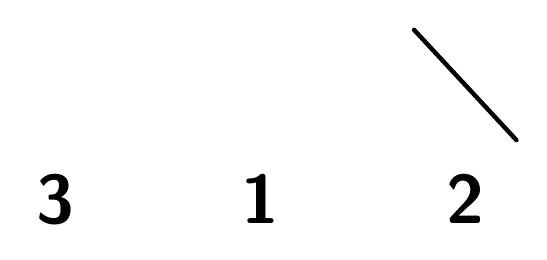
\begin{tikzpicture}
        \foreach \x/\m in {0/PKxanhla,2.6/PKdo,5.2/PKvang}{\GAqua{\x}{0}{0.6}{\m}}
        \draw[black,line width=1.6pt,line cap=round] (4.55,0.7) -- (5.85,-0.7);
        \begin{scope}[font=\sffamily\bfseries\fontsize{30}{30}\selectfont]
            \node at (0,-1.45) {3}; \node at (2.6,-1.45) {1}; \node at (5.2,-1.45) {2};
            \begin{scope}[shift={(1.3,-1.45)},scale=0.8]\GAdautru{black}\end{scope}
            \begin{scope}[shift={(3.9,-1.45)},scale=0.8]\GAdaubang{black}\end{scope}
        \end{scope}
    \end{tikzpicture}\par}
    \item GV giới thiệu phép trừ và dấu “$-$” gọi là dấu trừ, và hướng dẫn HS cách viết dấu trừ.
    \item HS luyện viết dấu trừ vào vở.
\end{itemize}
\newpage
\begin{luuy}
    \GAbs{\textbf{Mẹo giúp HS nhớ dấu trừ “$-$”:}
    \begin{itemize}\GAgon
        \item Dấu trừ giống \textbf{“chú sâu nằm ngủ”} hay \textbf{“que kem nằm ngang”} -- chỉ có \textbf{1 nét ngang}, nằm giữa dòng kẻ.
        \item \textbf{Viết theo thứ tự:} viết trên không $\to$ viết bằng ngón tay lên lưng bạn bên cạnh $\to$ viết bảng con $\to$ viết vào vở.
        \item \textbf{Câu vè:} \GAloi{Một nét ngang thôi, nằm ngay giữa dòng; bớt đi là trừ, các con nhớ không?}
    \end{itemize}}
\end{luuy}

%---------------------------------------------------------
\subsubsection{LUYỆN TẬP}
\begin{hd}
    \begin{itemize}\GAgon
        \item Thời gian: 10 phút
        \item HS gạch bớt để được số lượng theo yêu cầu, nói được câu “Có \dots, bớt \dots, còn lại \dots”.
    \end{itemize}
\end{hd}
\begin{itemize}\GAgon
    \item GV vẽ một số hình ảnh lên bảng và yêu cầu HS gạch bớt để được các số lượng mà GV yêu cầu.
\end{itemize}
\begin{vd}
    GV vẽ 5 hình vuông và yêu cầu HS gạch bớt để còn lại 3 hình vuông.
    \GAbatdauhinh
    {\centering
    \begin{tikzpicture}
        \foreach \k/\m in {0/PKxanhnuoc,1/PKvang,2/PKhong,3/PKxanhla,4/PKcam}{%
            \begin{scope}[shift={(1.4*\k,0)}]
                \shade[top color=\m!45,bottom color=\m!85,draw=\m!50!black,thick,rounded corners=2pt] (-0.5,-0.5) rectangle (0.5,0.5);
                \fill[white,opacity=0.45,rounded corners=1pt] (-0.4,0.28) rectangle (0.15,0.38);
                \ifnum\k>2 \GAgach{0.6}\fi
            \end{scope}}
        \node[anchor=west,font=\sffamily\Large] at (6.5,0) {$5 - 2 = 3$};
    \end{tikzpicture}\par}
\end{vd}
\begin{itemize}\GAgon
    \item \GAbs{\textbf{Trò chơi “Tiếp sức gạch bớt” (thi đua giữa 2 đội):} GV vẽ 2 hàng hình giống nhau (VD: 5 ngôi sao). GV đọc yêu cầu \GAloi{Còn lại 2 ngôi sao!}, mỗi đội cử 1 bạn chạy lên gạch bớt. Đội nào gạch đúng và nói được câu \GAloi{Có 5, bớt 3, còn lại 2} được cộng điểm.}
    \item \GAbs{\textbf{Trò chơi “Bé làm ảo thuật gia” (tuỳ thời gian):} GV hô \GAloi{Có 5 ngón tay -- cụp đi 2 ngón!}, HS giơ tay đáp án và đồng thanh nói số còn lại. Có thể mời HS lên làm “ảo thuật gia” ra đề cho cả lớp.}
    \item Nhấn mạnh phép trừ là \textbf{đếm số lượng còn lại, đếm bớt, bớt đi.}
    \item GV lựa chọn các bài tập phù hợp với học sinh.
\end{itemize}

%---------------------------------------------------------
\subsubsection{NGHỈ GIẢI LAO}
\begin{hd}
    \begin{itemize}\GAgon
        \item Thời gian: 10 phút
        \item Hát và nhảy theo bài hát \textit{Baby Shark}.
    \end{itemize}
\end{hd}
\noindent Link bài hát: \url{https://youtu.be/XqZsoesa55w?si=iYBG52x-gX1Z_Svv}

%---------------------------------------------------------
\newpage
\subsubsection{ CỦNG CỐ, DẶN BÀI TẬP VỀ NHÀ}
\begin{hd}
    \begin{itemize}\GAgon
        \item Thời gian: 10 phút
        \item HS nhắc lại nội dung bài học; GV kiểm tra kiến thức và giao BTVN.
    \end{itemize}
\end{hd}
\begin{itemize}\GAgon
    \item GV có thể tuỳ vào tình hình HS mỗi lớp để cho các BT phù hợp.
    \item \GAbs{\textbf{Tổng kết:} GV và HS cùng nhắc lại: \GAloi{Phép trừ là bớt đi, đếm phần còn lại; dấu trừ là một nét ngang.} Tuyên dương nhóm có nhiều điểm nhất.}

\end{itemize}

%%%%%%%%%%%%%%%%%%%%%%%%%%%%%%%%%%%%%%%%%%%%%%%%%%%%%%%%%%
%                  GIÁO ÁN TIẾNG VIỆT
%%%%%%%%%%%%%%%%%%%%%%%%%%%%%%%%%%%%%%%%%%%%%%%%%%%%%%%%%%
\newpage
\setcounter{subsection}{0}
\begin{center}
        {\color{mauchinh!120}\bfseries\Large CHỦ ĐỀ 14: LÀM QUEN VỚI ÂM D, Đ}\\[2pt]
\end{center}

\subsection{MỤC TIÊU}
\begin{itemize}\GAgon
    \item Học sinh làm quen âm d, đ.
    \item Học sinh tập viết chữ d, đ.
    \item \GAbs{Học sinh \textbf{phân biệt được chữ d và chữ đ} (chữ đ có thêm một nét ngang ngắn).}
    \item Học sinh nhận biết được tiếng có âm d, đ; nói được từ ngữ chứa tiếng có âm d, đ.

\end{itemize}

\subsection{TIẾN TRÌNH DẠY HỌC}
\begin{itemize}\GAgon
    \item Giáo án, bút bảng, PPT trình chiếu, PBT, tranh, bảng con, hình ảnh.
\end{itemize}

\subsubsection{ ÔN TẬP LẠI ÂM A, Ă, Â}
\begin{hd}
    \begin{itemize}\GAgon
        \item Thời gian: 15 phút
        \item HS đọc đúng, nhận diện nhanh âm a, ă, â và tiếng chứa các âm đó.
    \end{itemize}
\end{hd}
\begin{itemize}\GAgon
    \item GV cho HS ôn tập lại âm a, ă, â:
\end{itemize}
\GAbatdauhinh
{\centering
    \GAhangchu{A}{a}{\GAchuA}{4}\par\nopagebreak\vspace{6pt}
    \GAhangtranh{\begin{scope}[scale=0.95]\GAcahe\end{scope}}{c\GAgc{á}}
                {\GAanh{ba.png}{2.6cm}}{b\GAgc{a}}
                {\GAanh{ba2.png}{2.6cm}}{b\GAgc{à}}\par\vspace{6pt}
    \GAhangchu{Ă}{ă}{\GAchuAw}{4}\par\nopagebreak\vspace{6pt}
    \GAhangtranh{\GAanh{an.png}{2.3cm}}{\GAgc{ă}n}
                {\begin{scope}[shift={(0,-0.05)},scale=0.95]\GArang\end{scope}}{r\GAgc{ă}ng}
                {\begin{scope}[shift={(0,-1.15)},scale=1.15]\GAmang\end{scope}}{m\GAgc{ă}ng}\par\vspace{6pt}
    \GAhangchu{Â}{â}{\GAchuAa}{4}\par\nopagebreak\vspace{6pt}
    \GAhangtranh{\begin{scope}[shift={(-0.4,-0.25)},scale=0.9]\GAsau\end{scope}}{s\GAgc{â}u}
                {\begin{scope}[shift={(0,-0.15)},scale=0.95]\GAnam\end{scope}}{n\GAgc{ấ}m}
                {\GAanh{trau.png}{2.5cm}}{tr\GAgc{â}u}\par}
\begin{itemize}\GAgon
    \item GV cho HS đọc cá nhân.
    \item GV chia nhóm cho HS đọc.
    \item Nhóm nào đọc được các âm đã học sẽ được cộng 2 điểm.
    \item \GAbs{\textbf{Trò chơi “Ai tinh mắt?”:} GV giơ nhanh thẻ chữ a, ă, â theo thứ tự ngẫu nhiên, HS đọc to thật nhanh. Lần sau GV che bớt một phần thẻ (chỉ để lộ phần dấu) để HS đoán.}
\end{itemize}
\begin{luuy}
    \GAbs{\textbf{Mẹo giúp HS phân biệt a -- ă -- â:}
    \begin{itemize}\GAgon
        \item \textbf{a} là bạn “không đội mũ”; \textbf{ă} đội \textbf{“cái chén ngửa”}; \textbf{â} đội \textbf{“cái nón lá”}.
        \item \textbf{Động tác:} a -- hai tay ôm bụng tròn; ă -- hai tay khum dưới cằm như cái chén; â -- hai tay chụm trên đầu như cái nón.
    \end{itemize}}
\end{luuy}

%---------------------------------------------------------
\subsubsection{ LÀM QUEN ÂM D, Đ}
\begin{hd}
    \begin{itemize}\GAgon
        \item Thời gian: 20 phút
        \item HS đọc đúng âm d, đ; phân biệt được chữ d và chữ đ.
    \end{itemize}
\end{hd}
\begin{itemize}\GAgon
    \item GV giới thiệu về chữ d, đ.
    \item \GAbs{\textbf{“Hộp quà bí mật”:} GV lắc hộp, hỏi \GAloi{Trong hộp có gì nhỉ?} rồi lần lượt lấy ra \textbf{con dê} $\to$ HS nói “dê” $\to$ GV: “Tiếng \textbf{dê} có âm \textbf{d} đứng đầu”. Tiếp theo lấy ra \textbf{cái đèn} $\to$ “đèn” $\to$ âm \textbf{đ}. Mời HS lên thò tay vào hộp, lấy đồ vật và nói tên (dừa, dù, đũa, đá\dots).}
    \item \GAbs{\textbf{So sánh d và đ:} GV đặt 2 thẻ chữ cạnh nhau, hỏi: \GAloi{Hai chữ này giống và khác nhau ở đâu?} $\to$ Giống: đều có nét cong kín và nét móc ngược dài. Khác: \textbf{đ có thêm một nét ngang} -- \GAloi{chữ d đeo thêm chiếc thắt lưng thì thành chữ đ}.}
    \item GV hướng dẫn HS đọc âm d, đ và tiếng chứa âm d, đ.
    \item GV phát âm chữ d, đ ba lần, cho HS phát âm lại theo GV theo hình thức cả lớp.
    \item \GAbs{Luyện phát âm đa dạng hình thức: \textbf{cả lớp $\to$ tổ $\to$ nhóm $\to$ cá nhân}. Chơi \textbf{“Cô to -- trò nhỏ”}: GV đọc to thì HS đọc nhỏ, GV đọc nhỏ thì HS đọc to.}
    \item \GAbs{\textbf{Câu vè:} \GAloi{d d -- con dê kêu be be; đ đ -- đèn sáng cho bé xem.} HS vừa đọc vừa làm động tác (d: hai tay làm sừng dê; đ: hai tay xoè ra như đèn sáng).}
    \item \GAbs{\textbf{Tạo hình chữ (tuỳ thời gian):} Mỗi nhóm dùng dây len / đất nặn tạo chữ d, sau đó thêm một nét ngang để biến thành chữ đ.}
\end{itemize}
% Bài 1, Bài 2: y như PBT PRE1 Tuần 14
\GAdatlaibai
\begin{bt}
    Bé hãy đọc và khoanh vào âm \textbf{d} của các từ phía dưới.
    \TThinh[2.6cm]{p14_image20.png}
    \TTbatdauhinh
    {\centering
        \PKbontranh{d}{p14_de.png}{con dê}{p14_hatde.png}{hạt dẻ}{p14_quediem.png}{que diêm}{p14_conde2.png}{con dế}\hfill
        \begin{minipage}[b]{0.42\linewidth}\centering\PKghep{d}{ê}{dê}\\[8pt]\PKghep{d}{ế}{dế}\end{minipage}\par}
\end{bt}

\begin{bt}
    Bé hãy đọc và khoanh vào âm \textbf{đ} của các từ phía dưới.
    \TThinh[2.6cm]{p14_image23.png}
    \TTbatdauhinh
    {\centering
        \PKbontranh{đ}{p14_duong.png}{con đường}{p14_do.png}{con đò}{p14_cayda.png}{cây đa}{p14_hatdieu.png}{hạt điều}\hfill
        \begin{minipage}[b]{0.42\linewidth}\centering\PKghep{đ}{o}{đo}\\[8pt]\PKghep{đ}{ò}{đò}\end{minipage}\par}
\end{bt}

\newpage

\begin{itemize}\GAgon
    \item Bài tập áp dụng: Bài 1, 2 trong Phiếu bài tập.
\end{itemize}

%---------------------------------------------------------
\subsubsection{NHẬN BIẾT ĐƯỢC TIẾNG CÓ ÂM D, Đ}
\begin{hd}
    \begin{itemize}\GAgon
        \item Thời gian: 10 phút
        \item HS nghe -- nhận ra tiếng có âm d, đ; nói được từ ngữ chứa tiếng có âm d, đ.
    \end{itemize}
\end{hd}
\begin{itemize}\GAgon
    \item GV nói một số từ có chứa âm d, đ cho HS thi đua nhau nói lại các từ có âm d, đ đã nghe.
    \item \GAbs{\textbf{Trò chơi “Tai ai thính?”:} GV đọc từng từ, nếu từ có âm \textbf{d} HS \textbf{vỗ tay 1 cái}, nếu có âm \textbf{đ} HS \textbf{dậm chân 1 cái}. Từ gợi ý:}
\end{itemize}
{\centering
    \renewcommand{\arraystretch}{1.45}
    \begin{tabular}{|>{\centering\arraybackslash}p{6.5cm}|>{\centering\arraybackslash}p{6.5cm}|}
        \hline
        \textbf{Từ có âm d} & \textbf{Từ có âm đ}\\
        \hline
        dê, dừa, dù, dao & đèn, đá, đũa, đỏ\\
        \hline
        dế, da, dì, dưa & đu đủ, đậu, đồng hồ, đi\\
        \hline
    \end{tabular}\par}
\begin{itemize}\GAgon
    \item \GAbs{\textbf{“Ai nhanh hơn?”:} Hai đội thi kể tên đồ vật, con vật có âm d hoặc đ; mỗi từ đúng được 1 ngôi sao.}
    \item GV hướng dẫn HS thực hiện các bài tập trong PBT.
\end{itemize}

\textbf{1.} Bé hãy tô màu \textbf{xanh dương} vào giọt nước có từ chứa chữ \textbf{d} và tô màu \textbf{hồng} vào giọt nước có từ chứa chữ \textbf{đ}.
\GAbatdauhinh
{\centering
\begin{tikzpicture}[scale=1.15]
    \foreach \tu/\x/\y in {đi/0/0.2,dừa/1.9/-0.1,đua/3.8/0.15,dế/5.7/-0.15,đỏ/7.6/0.2,
                           dê/0.9/-2.3,đói/2.8/-2.0,đậu/4.7/-2.35,đi/6.6/-2.05,diều/8.5/-2.3}{
        \begin{scope}[shift={(\x,\y)}]\PKgiot{\tu}\end{scope}}
\end{tikzpicture}\par}
\medskip

\textbf{2.} Bé hãy nối tên với hình ảnh tương ứng nhé:
\GAbatdauhinh
{\centering
\begin{tikzpicture}
    \node[inner sep=0pt] at (0,2.4) {\GAhinhx[height=2.2cm]{duahau.png}};
    \node[inner sep=0pt] at (0,-0.4) {\GAhinhx[height=2.0cm]{hatdau.png}};
    \node[inner sep=0pt] at (11,2.4) {\GAhinhx[height=2.3cm]{dudu.png}};
    \node[inner sep=0pt] at (11,-0.4) {\GAhinhx[height=2.1cm]{quadua.png}};
    \foreach \y in {2.4,-0.4}{\fill (1.55,\y) circle (3pt); \fill (9.45,\y) circle (3pt);}
    \foreach \tu/\y in {quả dừa/2.7,đu đủ/1.5,dưa hấu/0.3,hạt đậu/-0.9}{%
        \node[draw,line width=1.2pt,rounded corners=5pt,fill=PKvangnhat,minimum width=3.2cm,minimum height=0.85cm,font=\Large] at (5.5,\y) {\tu};}
\end{tikzpicture}\par}
\medskip

\textbf{3.} Bé hãy viết và đọc các từ sau:
\GAbatdauhinh
{\centering
\begin{tikzpicture}
    % hàng 1: dê, cò
    \node[inner sep=0pt] at (1.0,0.55) {\GAhinhx[height=1.9cm]{conde_dung.png}};
    \GAdongviet{2.4}{0}{2.6}{dê}
    \node[inner sep=0pt] at (9.6,0.55) {\GAhinhx[height=1.9cm]{co.png}};
    \GAdongviet{11.0}{0}{2.6}{cò}
    \draw[PKdo!65,line width=1.8pt,dash pattern=on 6pt off 4pt] (-0.4,-0.85) -- (15.8,-0.85);
    % hàng 2: đá, ô tô
    \node[inner sep=0pt] at (1.0,-2.0) {\GAhinhx[width=2.4cm]{da.png}};
    \GAdongviet{2.4}{-2.5}{2.6}{đá}
    \begin{scope}[shift={(9.4,-2.05)},scale=0.72]\GAoto\end{scope}
    \GAdongviet{11.0}{-2.5}{3.6}{ô tô}
    \draw[PKdo!65,line width=1.8pt,dash pattern=on 6pt off 4pt] (-0.4,-3.35) -- (15.8,-3.35);
    % hàng 3: Đô có cá
    \node[inner sep=0pt] at (2.0,-5.0) {\GAhinhx[height=2.6cm]{beca.png}};
    \GAdongviet{5.0}{-5.4}{6.6}{Đô có cá}
\end{tikzpicture}\par}
\medskip

\textbf{4.} Nối tên các con vật với dấu phù hợp:
\GAbatdauhinh
{\centering
\begin{tikzpicture}[font=\bfseries\large]
    % hai dấu thanh ở giữa
    \node[draw,line width=1.5pt,circle,fill=PKvangnhat,minimum size=1.6cm] (n) at (-1.0,0) {};
    \begin{scope}[shift={(-1.0,0)}]\GAdaunang\end{scope}
    \node[draw,line width=1.5pt,circle,fill=green!15,minimum size=1.6cm] (g) at (1.0,0) {};
    \begin{scope}[shift={(1.0,0)}]\GAdaunga\end{scope}
    % các con vật: tên nút / vị trí / hình / tên / điểm nối (dưới tên, hoặc cạnh tranh)
    \foreach \t/\p/\h/\ten/\noi in {a1/{(-3.0,3.1)}/ngong.png/con ngỗng/{([yshift=-4pt]a1t.south)},
                                    a2/{(3.2,3.1)}/vuon.png/con vượn/{([yshift=-4pt]a2t.south)},
                                    a3/{(-5.8,0.2)}/vet.png/con vẹt/{([xshift=5pt]a3.east)},
                                    a4/{(5.8,0.2)}/bosua.png/bò sữa/{([xshift=-5pt]a4.west)},
                                    a5/{(0,-3.2)}/qua.png/con quạ/{([yshift=4pt]a5.north)}}{%
        \node[inner sep=0pt] (\t) at \p {\GAhinhx[height=1.7cm]{\h}};
        \node[anchor=north,inner sep=2pt] (\t t) at (\t.south) {\ten};
        \fill \noi circle (3pt);}
    % điểm nối trên hai dấu
    \foreach \p in {n.north,n.south,n.west,g.north,g.south,g.east}{\fill ([shift={(0,0)}]\p) circle (3pt);}
\end{tikzpicture}\par}

%---------------------------------------------------------
\subsubsection{ TẬP VIẾT CHỮ D, Đ}
\begin{hd}
    \begin{itemize}\GAgon
        \item Thời gian: 25 phút
        \item HS nắm cấu tạo, cách viết và viết đúng chữ d, đ.
    \end{itemize}
\end{hd}
\begin{itemize}\GAgon
    \item GV viết mẫu chữ d, đ lên bảng vừa viết vừa nói cách viết: phân tích cấu tạo chữ d, đ.
\end{itemize}
{\renewcommand{\arraystretch}{1.25}
\noindent\begin{tabular}{|m{0.66\linewidth}|>{\centering\arraybackslash}m{0.26\linewidth}|}
    \hline
    \textbf{-- Cấu tạo:} Chữ d cao 4 ly, rộng 2,5 ly. Gồm 2 nét: nét cong kín và nét móc ngược dài ở bên phải.\newline
    \textbf{-- Cách viết:}\newline
    \textbf{\textit{+ Nét cong kín:}} Đặt bút dưới đường kẻ ngang 3 một chút, viết nét cong kín từ phải sang trái, dừng bút ở điểm xuất phát.\newline
    \textbf{\textit{+ Nét móc ngược dài:}} Từ điểm dừng bút của nét 1, lia bút lên đường kẻ ngang 5 viết nét móc ngược dài ở bên phải, sát nét cong kín, đến góc đường kẻ ngang 2 thì dừng lại.
    & \vspace{4pt}\GAquytrinh{}{}\vspace{4pt}\\
    \hline
    \textbf{-- Cấu tạo:} Chữ đ cao 4 ly, rộng 2,5 ly. Gồm 3 nét: nét cong kín, nét móc ngược dài ở bên phải và nét ngang ngắn.\newline
    \textbf{-- Cách viết:}\newline
    \textbf{\textit{+ Nét cong kín:}} Đặt bút dưới đường kẻ ngang 3 một chút, viết nét cong kín từ phải sang trái, dừng bút ở điểm xuất phát.\newline
    \textbf{\textit{+ Nét móc ngược dài:}} Từ điểm dừng bút của nét 1, lia bút lên đường kẻ ngang 5 viết nét móc ngược dài ở bên phải, sát nét cong kín, đến góc đường kẻ ngang 2 thì dừng lại.\newline
    \textbf{\textit{+ Nét ngang ngắn:}} Từ điểm dừng bút của nét 2 thì lia bút lên đường kẻ ngang 4 tại điểm giữa đường kẻ dọc 2 và 3, viết 1 nét ngang ngắn từ trái sang phải, dừng bút tại điểm giữa đường kẻ dọc 3 và 4.
    & \vspace{4pt}\GAquytrinh{\fill (1.5,2.94) rectangle (2.5,3.07);}{\draw[-stealth] (1.0,2.68) -- (1.6,2.68); \node at (1.2,3.05) {3};}\vspace{4pt}\\
    \hline
\end{tabular}\par}
\begin{itemize}\GAgon
    \item GV cho HS nhắc lại.
    \item \GAbs{\textbf{Trước khi viết bảng con:} HS viết chữ d, đ \textbf{trên không} theo tay cô, rồi viết bằng ngón tay lên \textbf{lưng bạn} bên cạnh, bạn đoán chữ gì.}
    \item \GAbs{\textbf{Nhắc tư thế ngồi viết qua câu vè:} \GAloi{Lưng thẳng, mắt xa một gang, tay trái tì vở, tay phải cầm bút ngay hàng.}}
    \item HS viết mẫu vào bảng con.
    \item HS viết nhanh và đẹp sẽ được điểm cộng.
    \item GV cho HS tập viết chữ d, đ trong Phiếu bài tập.
    \item \GAbs{GV đi quan sát, cầm tay hướng dẫn HS còn lúng túng; gắn sticker \textbf{“Bàn tay khéo”} cho bài viết đẹp.}
\end{itemize}

%---------------------------------------------------------
\subsubsection{CỦNG CỐ VÀ GIAO BÀI TẬP VỀ NHÀ}
\begin{hd}
    \begin{itemize}\GAgon
        \item Thời gian: 10 phút
        \item GV giao BTVN phù hợp với tình hình HS lớp mình.
    \end{itemize}
\end{hd}
\begin{itemize}\GAgon
    \item \GAbs{\textbf{Trò chơi củng cố “Ong tìm hoa”:} GV dán các bông hoa có từ (dê, đèn, dừa, đá\dots) lên bảng; 2 chú ong mang chữ \textbf{d} và \textbf{đ}. HS lên gắn bông hoa về đúng chú ong của mình. Cả lớp kiểm tra và đọc lại.}
    \item \GAbs{\textbf{Tổng kết:} Cả lớp đọc lại câu vè d -- đ, GV tuyên dương nhóm / cá nhân tích cực.}
    \item \GAbs{\textbf{Gợi ý BTVN vui:} Bé tìm 3 đồ vật trong nhà có âm d hoặc đ (VD: đũa, đèn, dép) và kể cho ba mẹ nghe.}
\end{itemize}

\begin{center}
       \faGg\faGg\quad Hết \quad\faGg\faGg
\end{center}
\end{document}
